%%%%%%%%%%%%%%%%%%%%%%%%%%%%%%%%%%%%%%%%%
% Masters/Doctoral Thesis 
% LaTeX Template
% Version 2.5 (27/8/17)
%
% This template was downloaded from:
% http://www.LaTeXTemplates.com
%
% Version 2.x major modifications by:
% Vel (vel@latextemplates.com)
%
% This template is based on a template by:
% Steve Gunn (http://users.ecs.soton.ac.uk/srg/softwaretools/document/templates/)
% Sunil Patel (http://www.sunilpatel.co.uk/thesis-template/)
%
% Template license:
% CC BY-NC-SA 3.0 (http://creativecommons.org/licenses/by-nc-sa/3.0/)
%
%%%%%%%%%%%%%%%%%%%%%%%%%%%%%%%%%%%%%%%%%

%----------------------------------------------------------------------------------------
%	PACKAGES AND OTHER DOCUMENT CONFIGURATIONS
%----------------------------------------------------------------------------------------

\documentclass[
11pt, % The default document font size, options: 10pt, 11pt, 12pt
%oneside, % Two side (alternating margins) for binding by default, uncomment to switch to one side
english, % ngerman for German
singlespacing, % Single line spacing, alternatives: onehalfspacing or doublespacing
openany, % Remove blank page after chapters
%draft, % Uncomment to enable draft mode (no pictures, no links, overfull hboxes indicated)
%nolistspacing, % If the document is onehalfspacing or doublespacing, uncomment this to set spacing in lists to single
%liststotoc, % Uncomment to add the list of figures/tables/etc to the table of contents
%toctotoc, % Uncomment to add the main table of contents to the table of contents
%parskip, % Uncomment to add space between paragraphs
%nohyperref, % Uncomment to not load the hyperref package
headsepline, % Uncomment to get a line under the header
%chapterinoneline, % Uncomment to place the chapter title next to the number on one line
%consistentlayout, % Uncomment to change the layout of the declaration, abstract and acknowledgements pages to match the default layout
]{MastersDoctoralThesis} % The class file specifying the document structure

\usepackage[utf8]{inputenc} % Required for inputting international characters
\usepackage[T1]{fontenc} % Output font encoding for international characters

\usepackage{mathpazo} % Use the Palatino font by default

\usepackage[backend=bibtex,style=authoryear,natbib=true]{biblatex} % Use the bibtex backend with the authoryear citation style (which resembles APA)

\addbibresource{phd_diary.bib} % The filename of the bibliography

\usepackage[autostyle=true]{csquotes} % Required to generate language-dependent quotes in the bibliography
\usepackage[section]{placeins}
\usepackage[section]{placeins}
\usepackage{multirow}
\usepackage[none]{hyphenat}
\usepackage[table]{colortbl}% http://ctan.org/pkg/xcolor
%----------------------------------------------------------------------------------------
%	MARGIN SETTINGS
%----------------------------------------------------------------------------------------

\geometry{
	paper=a4paper, % Change to letterpaper for US letter
	inner=2.5cm, % Inner margin
	outer=3.8cm, % Outer margin
	bindingoffset=.5cm, % Binding offset
	top=1.5cm, % Top margin
	bottom=1.5cm, % Bottom margin
	%showframe, % Uncomment to show how the type block is set on the page
}

%----------------------------------------------------------------------------------------
%	THESIS INFORMATION
%----------------------------------------------------------------------------------------

\thesistitle{Calibration in Cost-Effectiveness modeling (research diary)} % Your thesis title, this is used in the title and abstract, print it elsewhere with \ttitle
\supervisor{ Dr. Josep Lluis \textsc{Arcos} \\ Dr. Mireia \textsc{Díaz}} % Your supervisor's name, this is used in the title page, print it elsewhere with \supname
\examiner{} % Your examiner's name, this is not currently used anywhere in the template, print it elsewhere with \examname
\degree{Doctor of Philosophy} % Your degree name, this is used in the title page and abstract, print it elsewhere with \degreename
\author{David \textsc{Gómez}} % Your name, this is used in the title page and abstract, print it elsewhere with \authorname
\addresses{} % Your address, this is not currently used anywhere in the template, print it elsewhere with \addressname

\subject{Biological Sciences} % Your subject area, this is not currently used anywhere in the template, print it elsewhere with \subjectname
\keywords{} % Keywords for your thesis, this is not currently used anywhere in the template, print it elsewhere with \keywordnames
\university{\href{https://www.uab.cat}{Universitat Autònoma de Barcelona}} % Your university's name and URL, this is used in the title page and abstract, print it elsewhere with \univname
\department{\href{https://www.uab.cat/enginyeria/}{Escola d'Enginyeria de la UAB}} % Your department's name and URL, this is used in the title page and abstract, print it elsewhere with \deptname
\group{\href{https://www.iiia.csic.es/en-us/}{Artificial Intelligence Research Institute (IIIA)}} % Your research group's name and URL, this is used in the title page, print it elsewhere with \groupname
\faculty{\href{http://faculty.university.com}{Faculty Name}} % Your faculty's name and URL, this is used in the title page and abstract, print it elsewhere with \facname

\AtBeginDocument{
\hypersetup{pdftitle=\ttitle} % Set the PDF's title to your title
\hypersetup{pdfauthor=\authorname} % Set the PDF's author to your name
\hypersetup{pdfkeywords=\keywordnames} % Set the PDF's keywords to your keywords
}

\begin{document}

\frontmatter % Use roman page numbering style (i, ii, iii, iv...) for the pre-content pages

\pagestyle{plain} % Default to the plain heading style until the thesis style is called for the body content

\begin{titlepage}
	\begin{center}
		
		\vspace*{.06\textheight}
		{\scshape\LARGE \univname\par}\vspace{1.5cm} % University name
		\textsc{\Large Doctoral Thesis}\\[0.5cm] % Thesis type
		
		\HRule \\[0.4cm] % Horizontal line
		{\huge \bfseries \ttitle\par}\vspace{0.4cm} % Thesis title
		\HRule \\[1.5cm] % Horizontal line
		
		\begin{minipage}[t]{0.4\textwidth}
			\begin{flushleft} \large
				\emph{Author:}\\
				\href{}{\authorname} % Author name - remove the \href bracket to remove the link
			\end{flushleft}
		\end{minipage}
		\begin{minipage}[t]{0.4\textwidth}
			\begin{flushright} \large
				\emph{Supervisors:} \\
				\href{}{\supname} % Supervisor name - remove the \href bracket to remove the link  
			\end{flushright}
		\end{minipage}\\[3cm]
		
		\vfill
		
		\large \textit{A thesis submitted in fulfillment of the requirements\\ for the degree of \degreename}\\[0.3cm] % University requirement text
		\textit{in the}\\[0.4cm]
		\groupname\\\deptname\\[2cm] % Research group name and department name
		
		\vfill
		
		{\large \today}\\[4cm] % Date
		%\includegraphics{Logo} % University/department logo - uncomment to place it
		
		\vfill
	\end{center}
\end{titlepage}

%----------------------------------------------------------------------------------------
%	LIST OF CONTENTS/FIGURES/TABLES PAGES
%----------------------------------------------------------------------------------------

\tableofcontents % Prints the main table of contents

%----------------------------------------------------------------------------------------
%	THESIS CONTENT - CHAPTERS
%----------------------------------------------------------------------------------------

\mainmatter % Begin numeric (1,2,3...) page numbering

\pagestyle{thesis} % Return the page headers back to the "thesis" style

% Include the chapters of the thesis as separate files from the Chapters folder
% Uncomment the lines as you write the chapters

% Chapter 1

\chapter{Background} % Main chapter title

\label{sec:background} % For referencing the chapter elsewhere, use \ref{Chapter1} 

%----------------------------------------------------------------------------------------

% Define some commands to keep the formatting separated from the content 
\newcommand{\keyword}[1]{\textbf{#1}}
\newcommand{\tabhead}[1]{\textbf{#1}}
\newcommand{\code}[1]{\texttt{#1}}
\newcommand{\file}[1]{\texttt{\bfseries#1}}
\newcommand{\option}[1]{\texttt{\itshape#1}}

%----------------------------------------------------------------------------------------

\section{Cost-Effectiveness Models in Healthcare}

\subsection{Objective}
Compare different strategies for detection/treatment of a disease, from health and economic point of view.

\subsection{Methodology}
Simulation model to mimic the strategies and compare the outputs for each strategy to determine which strategies are worth considering. A special ``strategy'' called the natural history describes the progression of the disease without any planned interventions, and it is used to calibrate some the inputs that will be used in the rest of strategies (see section \ref{sec:calibration}).

\begin{figure}[h]
	\centering
	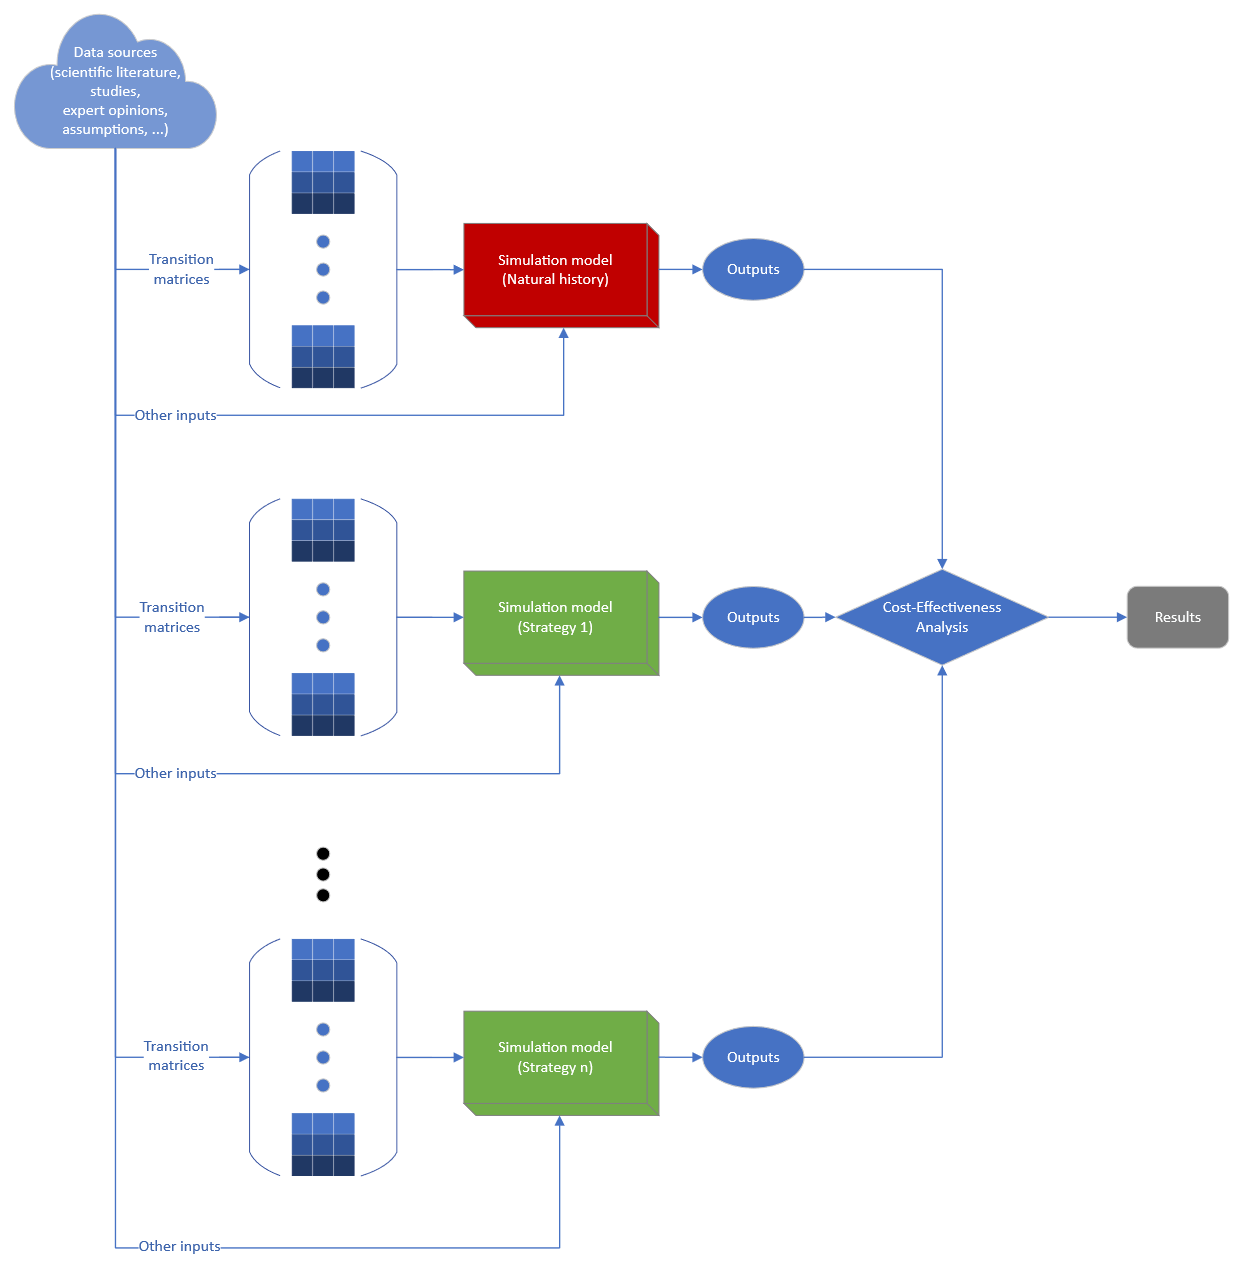
\includegraphics[width=\textwidth]{figures/cea_overview}
	\decoRule
	\caption[CEA overview]{Overview of the cost-effectiveness analysis.}
	\label{fig:cea_overview}
\end{figure}

\subsection{Types of model}
Decision trees, markov model, microsimulation, ... depending on the needs of the domain and the degree of detail and granularity required.

\begin{figure}[h]
	\centering
	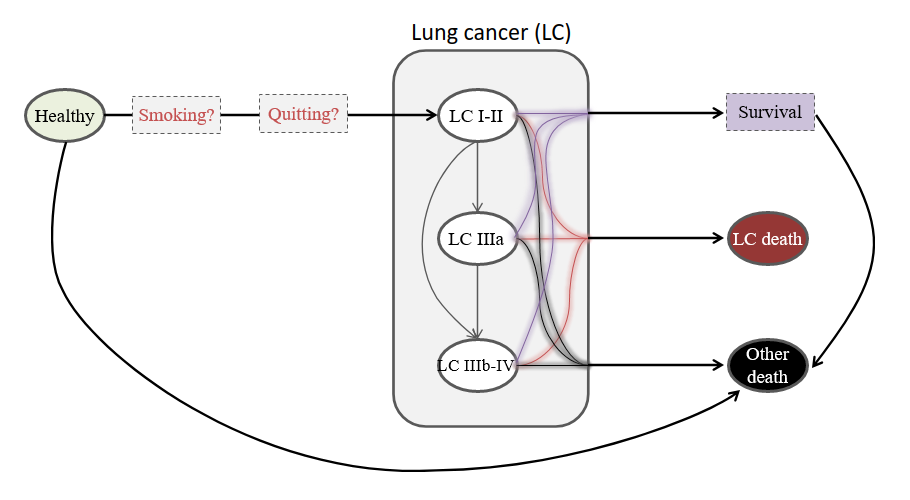
\includegraphics[width=\textwidth]{figures/lung_markov}
	\decoRule
	\caption[Markov state diagram]{Markov state diagram of the lung cancer model.}
	\label{fig:lung_markov}
\end{figure}

\subsection{Inputs}
Parameters extracted from the scientific literature, studies, expert opinions, assumptions, ... An interesting intermediate input are the transition matrices that show the probabilities of transitioning between health states.

\subsection{Outputs}
For each strategy:
\begin{itemize}
\item Effectiveness measure (e.g. Quality-Adjusted Life Years, QALYs)
\item Cost measure (e.g. euros, €)
\item Other general measures of interest: incidence, mortality, ...
\item Other domain-dependent measures: e.g. number of hysterectomies, number of high-grade lesions, ...
\end{itemize}


%----------------------------------------------------------------------------------------


% Chapter 1

\chapter{Cost-Effectiveness Analysis Methodology} % Main chapter title

\label{sec:methodology} % For referencing the chapter elsewhere, use \ref{Chapter1} 

\section{Calibration}
Before starting the base analysis, we calibrate the transition matrices in the natural history by slightly modifying the original probabilities so that the output of our model (e.g. incidence, mortality, …) fits an observed value based on evidence. These calibrated probabilities can then be used by the rest of the strategies in the base analysis. See Calibration Workflow for more details.

\begin{figure}[h]
	\centering
	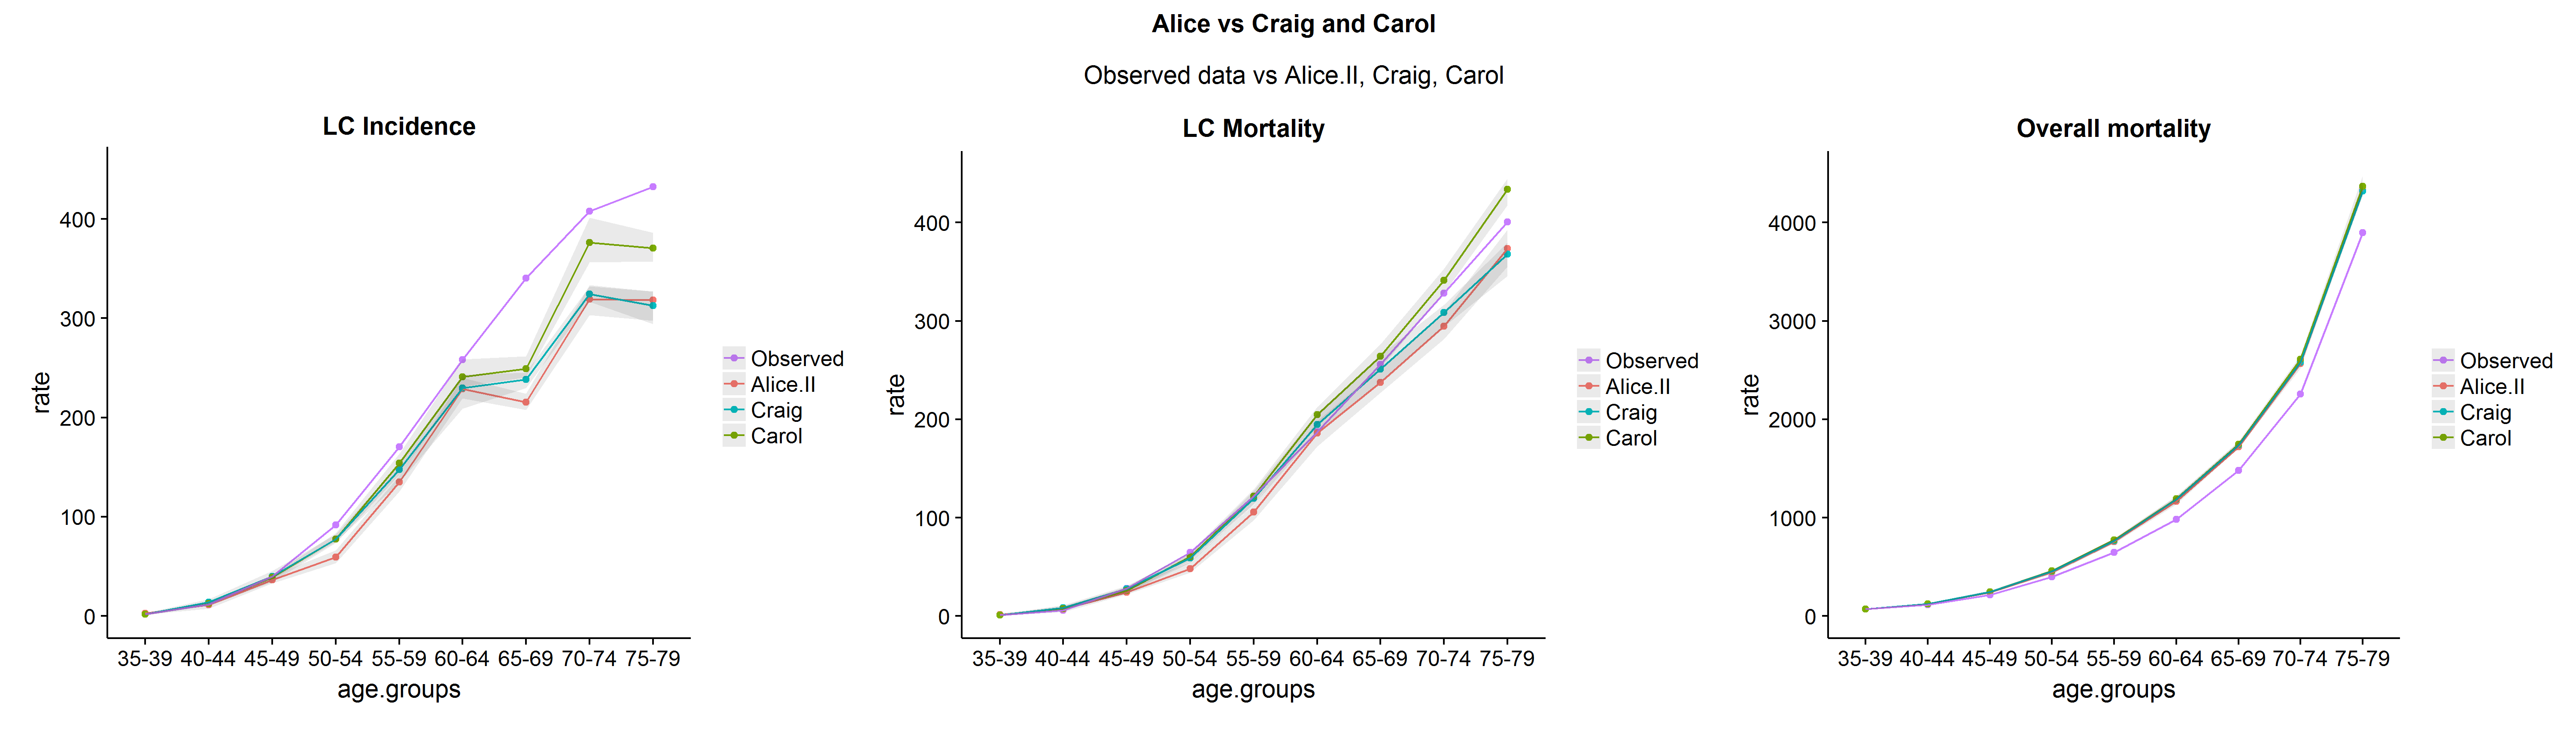
\includegraphics[width=\textwidth]{figures/lung_calibration_curves}
	\decoRule
	\caption[Calibration curve examples]{Example of three calibration curves for incidence, lung cancer mortality and mortality from other causes, along with the expected outcome.}
	\label{fig:lung_calibration_curves}
\end{figure}

\section{Base analysis}
Each strategy is plotted in the Cost and Effectiveness axes and the efficiency curve shows the strategies that are cost-effective, the rest are dominated by them and they are not considered cost-effective.

\begin{figure}[h]
	\centering
	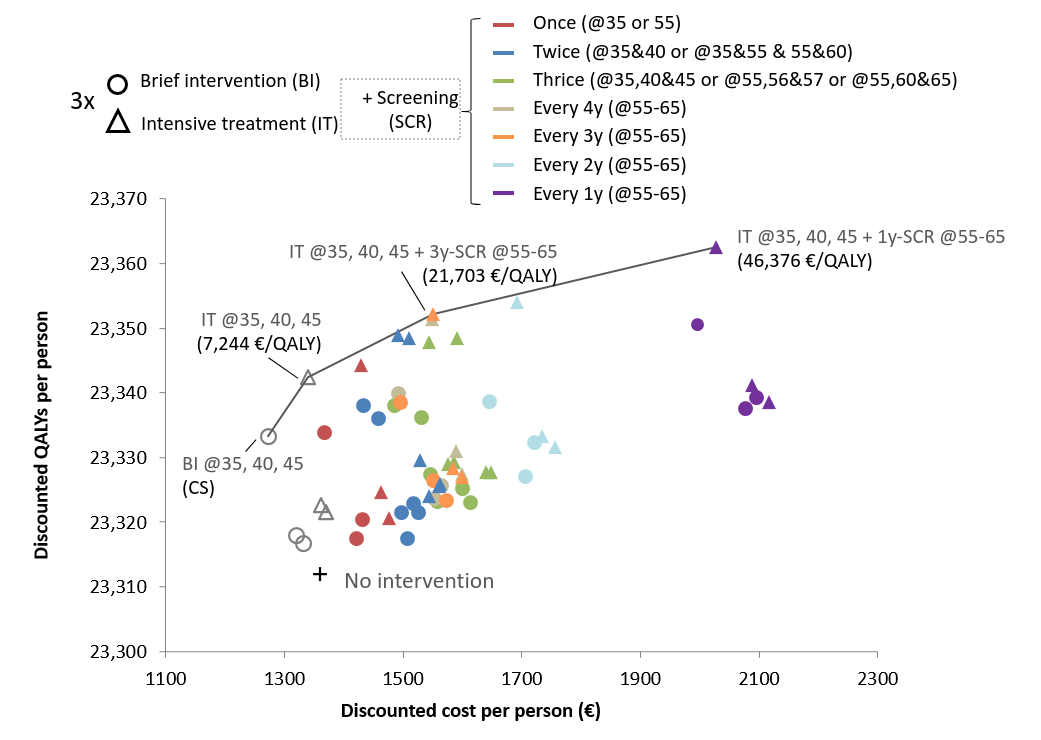
\includegraphics[width=\textwidth]{figures/lung_efficiency_curve}
	\decoRule
	\caption[Efficiency curve example]{Example of an efficiency curve showing the cost (€) and effectiveness (QALYs) of each of the simulated strategies. The strategies on the curve represent the cost-effective strategies, those below it are not usually considered since they are always dominated by one of those in the curve.}
	\label{fig:lung_efficiency_curve}
\end{figure}

We can compare each strategy in relation to another calculating the Incremental Cost-Effectiveness Ratio as:

$$
ICER=\frac{\Delta C}{\Delta E} = \frac{C_2-C_1}{E_2-E_1}
$$

If the ICER is below the Willingness-To-Pay (WTP) threshold (i.e. the maximum amount of money a country/region is willing to pay per additional QALY) the second strategy is more cost-effective than the first. If the ICER is greater than the WTP the strategy’s benefits are not considered cost-effective (i.e. the increased health benefit does not justify the increment of cost). Negative ICERs imply that one strategy dominates the other one.

\section{Sensitivity analysis}
Once the base analysis is performed we evaluate the uncertainty of the used parameters to check the robustness of the results. We modify the values of the parameters of interest to see how they affect the output of the model.

\subsection{Deterministic Sensitivity Analysis (DSA)}
A sweep is performed over a range (e.g. +-15\% of the base value) for the parameters of interest, to see how the ICER changes and whether the cost-effectiveness decision is different.

\begin{figure}[h]
	\centering
	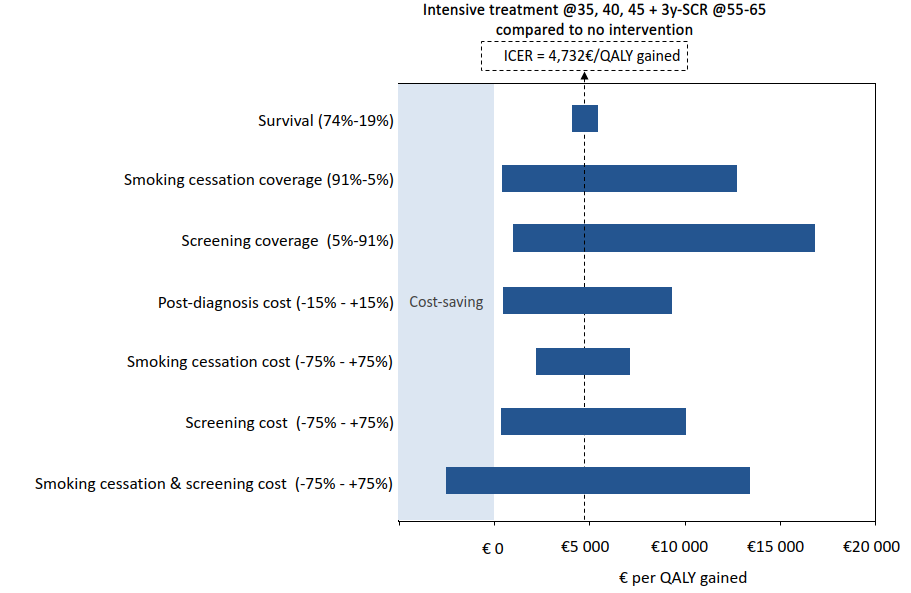
\includegraphics[width=\textwidth]{figures/lung_tornado}
	\decoRule
	\caption[Tornado diagram example]{Example of a tornado diagram showing the impact on the ICER between two particular strategies when changing one single parameter over a predefined range.}
	\label{fig:lung_tornado}
\end{figure}

\subsection{Probabilistic Sensitivity Analysis (PSA)}
Each parameter of interest is modeled as a probabilistic distribution (e.g. Beta for probabilities, Gamma/Lognormal for costs, ...) with the base value as the mean and a standard deviation dependent on the amount of uncertainty. We sample from these distributions (univariate or multivariate) to run a number of random simulations to check the percentage of simulations that show a cost-effective result (i.e. the percentage of simulations below the line ICER=WTP, see figure \ref{fig:endometrium_psa_scatterplot}).

\begin{figure}[h]
	\centering
	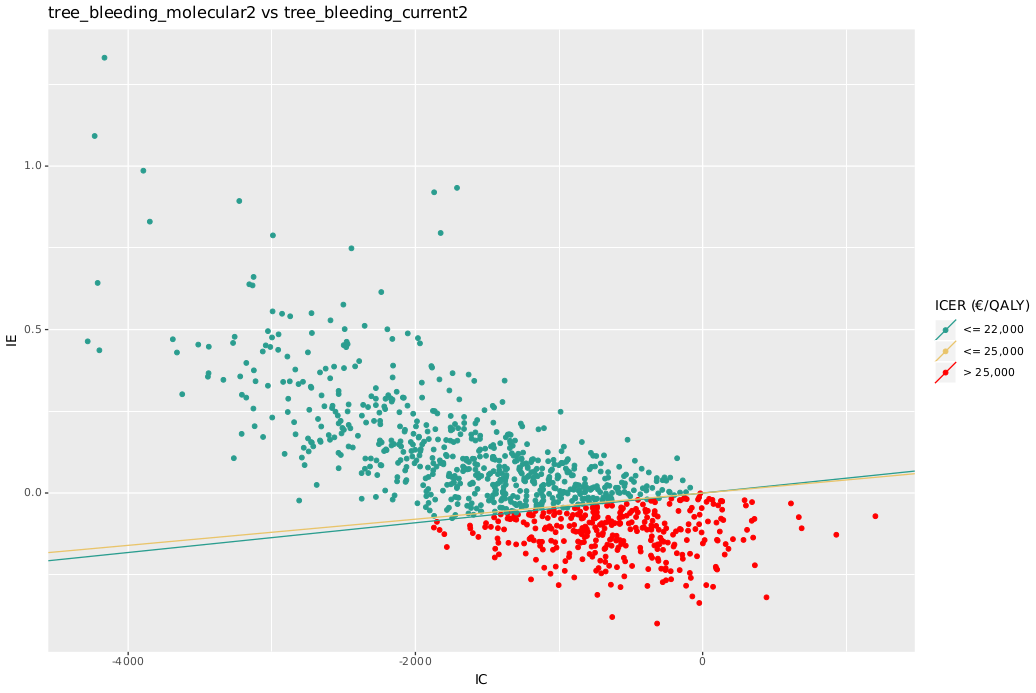
\includegraphics[width=\textwidth]{figures/endometrium_psa_scatterplot}
	\decoRule
	\caption[PSA scatterplot example]{Example of a scatterplot of a PSA, showing results from 1,000 random iterations and how they relate to the cost-effectiveness threshold (WTP). Green and red points represent cost-effective and non-cost-effective simulations respectively.}
	\label{fig:endometrium_psa_scatterplot}
\end{figure} 
% Chapter 1

\chapter{Calibration workflow} % Main chapter title

\label{sec:calibration} % For referencing the chapter elsewhere, use \ref{Chapter1} 

\begin{figure}[h]
	\centering
	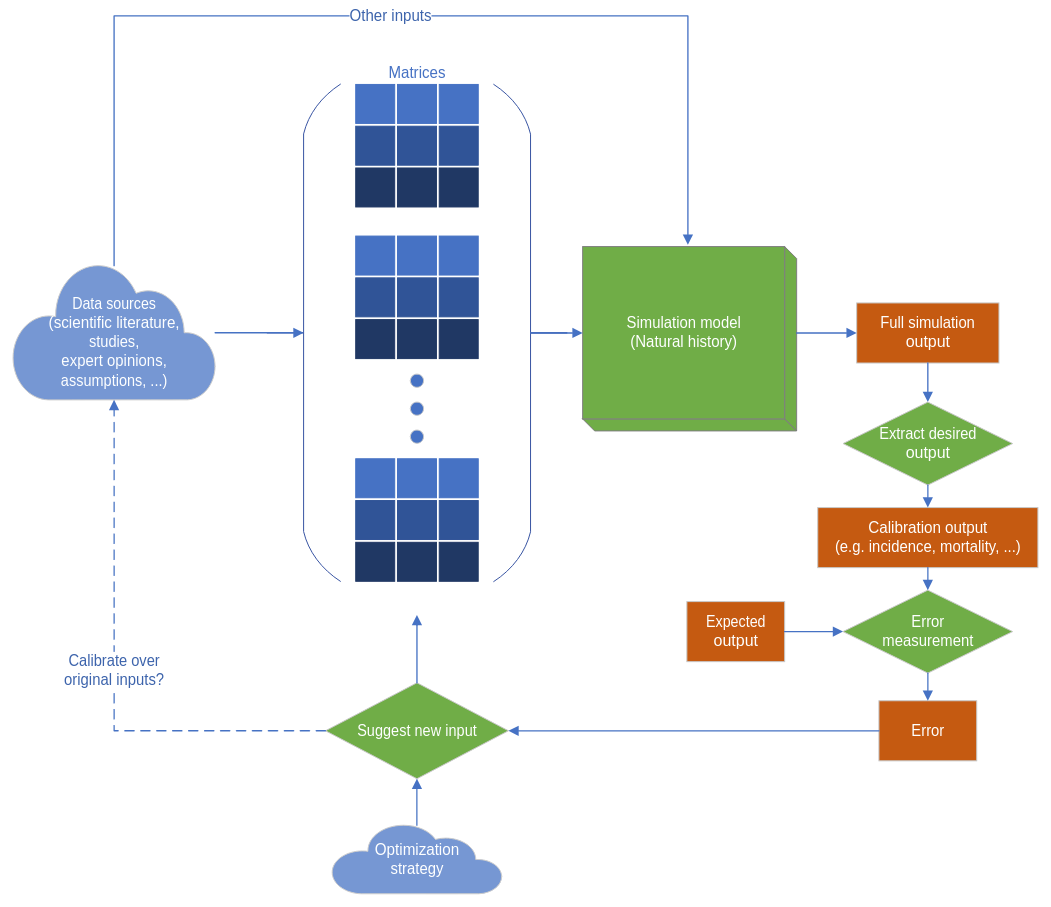
\includegraphics[width=\textwidth]{figures/calibration_workflow}
	\decoRule
	\caption[Calibration workflow]{Conceptual summary of the calibration procedure.}
	\label{fig:calibration_workflow}
\end{figure}


% Chapter 1

\chapter{Research proposal} % Main chapter title

\label{sec:proposal} % For referencing the chapter elsewhere, use \ref{Chapter1} 

Cost-effectiveness models are used to evaluate and compare different medical strategies (e.g. strategies to detect cancer), in terms of both health and cost, and to help decision makers determine the optimal allocation of medical resources. These models have several inputs that describe the environment, the disease and the strategies used (inputs like probabilities, sensitivities and specificities for medical procedures, costs, utility values, ...) and can have several outputs as needed for the analysis (e.g. average life expectancy, average cost, incidence of the disease, mortality, ...). 

The stated goal of the research project is to find efficient ways to calibrate these cost-effectiveness models by changing some input parameters so a particular output (usually incidence or mortality) matches a given value found in the scientific literature. In summary, \textbf{we can frame the problem as the optimization of a black box function computing (for example) the euclidean distance between the simulated output and a theoretical value}.

In some of our models we find that classical optimization methods need many simulations to converge to a good solution, demanding a lot of time and computing resources. Also, in many cases we are able to provide information about the statistical distribution of some of the inputs that could help in the optimization process. For these reasons I believe Bayesian Optimization (BO) might be a good alternative to adapt to our particular modeling needs.

Some preliminary (ongoing) experiments, using both bayesian and classical methods, are available in a jupyter notebook in \url{https://github.com/david-gomez-guillen/phd}, using the hypermapper [\cite{proposal:hypermapper}] python library for BO and scipy for classical optimization methods. This first set of tests focus on the performance of different optimization methods on well-known analytical functions that are easy to compute. Once acquainted with BO usage, the next step would be to repeat the tests on the actual cost-effectiveness models.

The conclusions and challenges found in the tests so far include:
\begin{enumerate}
	\item BO using Gaussian Processes might be too slow for some of our more lightweight simulation models, classical methods converge faster even if they need more function evaluations. It should not be a problem for more computationally expensive simulation models.
	\item BO tests performed converge to worse optima compared to classical optimization methods (e.g. Nelder-Mead, BFGS). It might be due to code issues: either implementation problems or an incorrect usage of the library.
	\item Gaussian processes regression used in BO becomes more expensive for each iteration due to having to calculate the inverse of a matrix that grows with the number of observations. Regression becomes very slow to compute after a number of evaluations, especially for high-dimensional inputs (depending on the available hardware) [\cite{proposal:fast_gaussian}][\cite{proposal:splitting_gaussian}].
	\item Regular bayesian methodology (updating iteratively the model after each observation) is more difficult to parallelize than classical methods, though some alternatives exist [\cite{proposal:parallel_bayesian}][\cite{proposal:parallel_bayesian2}].
	\item BO in these tests performed with priors for the optimum [\cite{souza_bayesian_2021}] (implemented in hypermapper: \url{https://github.com/luinardi/hypermapper/wiki/prior-injection}) do not seem to converge faster. It might be due to library issues too: optimum priors implementation is labeled as experimental in the documentation.
	\item When optimizing the actual cost-effectiveness models in future tests it would be interesting to add constraints for the inputs [\cite{gardner_bayesian_nodate}][\cite{ungredda_bayesian_2021}]. E.g: one input parameter being greater than another.
\end{enumerate}
% Chapter 1

\chapter{Thoughts \& ideas} % Main chapter title

\label{sec:ideas} % For referencing the chapter elsewhere, use \ref{Chapter1} 

\section{Sequential Model-Based Optimization (SMBO)}
Current tests are performed using regular Bayesian Optimization (BO) via Gaussian Processes. Resources are available in \url{src/R} (interactive demo code), \url{notebooks} (jupyter notebooks for the same demos) and \url{output/gp} (output plots for different regression scenarios).

\begin{figure}[h]
	\centering
	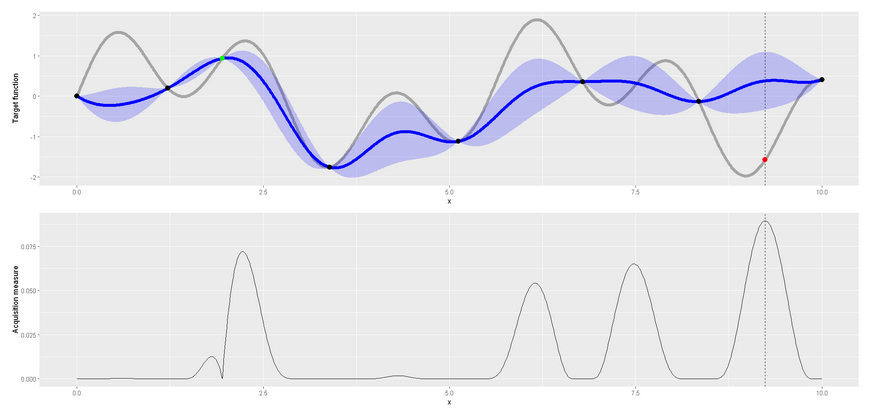
\includegraphics[width=\textwidth]{figures/bo_gp_regression}
	\decoRule
	\caption[Bayesian Optimization]{Bayesian Optimization using a Gaussian process after the eighth observed point. The acquisition function used is the Expected Improvement.}
	\label{fig:bo_gp_regression}
\end{figure}

The error functions that we are trying to optimize, though, are not particularly time-consuming, so other more naive approaches work better by producing good results in a much shorter time (though many more evaluations of the error function). In order to improve this method for these use cases we can focus on different areas.

\subsection{Surrogate model}
Bayesian Optimization uses a surrogate model to approximate the target function and determine the optimal candidates to evaluate for each iteration. The default choice in many cases is a Gaussian Process but other alternatives exist, such as random forests or Tree Parzen Estimators (TPE) [\cite{rasmussen_gaussian_2006}][\cite{bergstra_algorithms_2011}].

\subsection{Kernel selection/composition}
One crucial hyperparameter in the BO method is the kernel. This function determines how the uncertainty over the regression curve is determined and its properties can greatly influence the fit and inference performance of the surrogate model (figure \ref{fig:bo_gp_kernel}). An important step in the optimization procedure will be the selection and/or composition of kernels for the optimization problem [\cite{repicky_automated_nodate}][\cite{duvenaud_automatic_nodate}][\cite{duvenaud_additive_2011}][\cite{duvenaud_structure_2013}].

\begin{figure}[h]
	\centering
	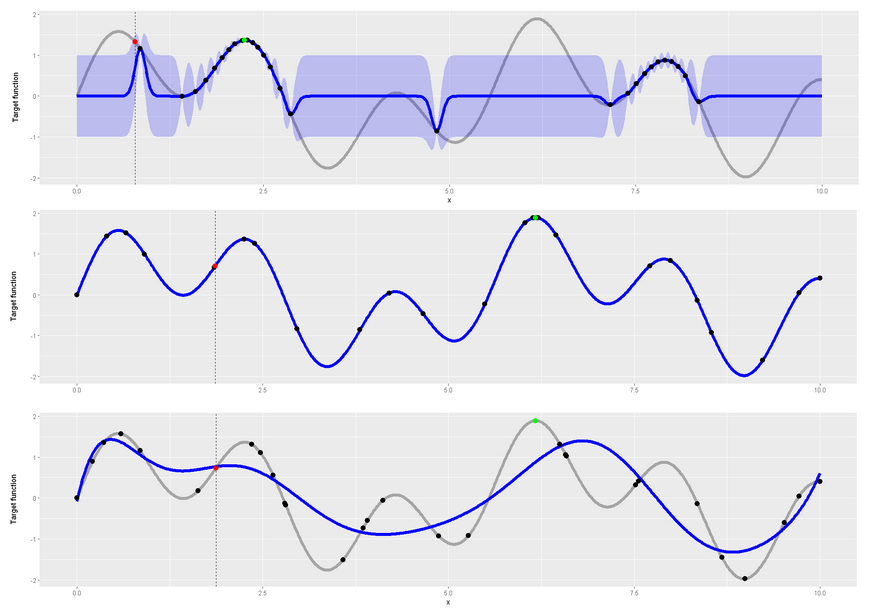
\includegraphics[width=\textwidth]{figures/bo_gp_kernel}
	\decoRule
	\caption[GP kernels]{Three GP regressions with different kernels $K(x,x')$ over the same target function: $e^{-100(x-x')^2}$ (top), $e^{-(x-x')^2}$ (middle) and $e^{-0.1(x-x')^2}$ (bottom). In the top plot each point has small influence over the rest, sampling new points inefficiently and resembling other local optimization techniques. In the bottom plot each point has too much small influence over the rest making a good fit impossible if the data varies more than expected. In the middle plot we can see a good fit with an appropriate kernel for the target function.}
	\label{fig:bo_gp_kernel}
\end{figure}

\begin{itemize}
\item \url{https://www.cs.toronto.edu/~duvenaud/cookbook/}
\item \url{https://nipunbatra.github.io/blog/ml/2021/09/03/param-learning-sgd.html}
\end{itemize}

\subsection{Batch iterations}
Each iteration we can select more than one candidate to evaluate. In expensive target functions this might be prohibitive, but in our case we might benefit for adding more information to the model. The batch size can be a modulation parameter depending on the computational cost of the function.

In the case of batches of more than one, we have to consider how those candidates are chosen: the maximum of the acquisition function is one, but the rest should be chosen such that the information provided is significant and not redundant given the rest (e.g. not too close to each other) [\cite{nguyen_budgeted_2017}][\cite{gonzalez_batch_nodate}].

\subsection{Constraints}

We suggest the use of the Constrained Expected Improvement acquisition function to incorporate constraints in the BO method [\cite{gardner_bayesian_nodate}]. An example can be seen in figure \ref{fig:bo_gp_regression_constraints}.

\begin{figure}[h]
	\centering
	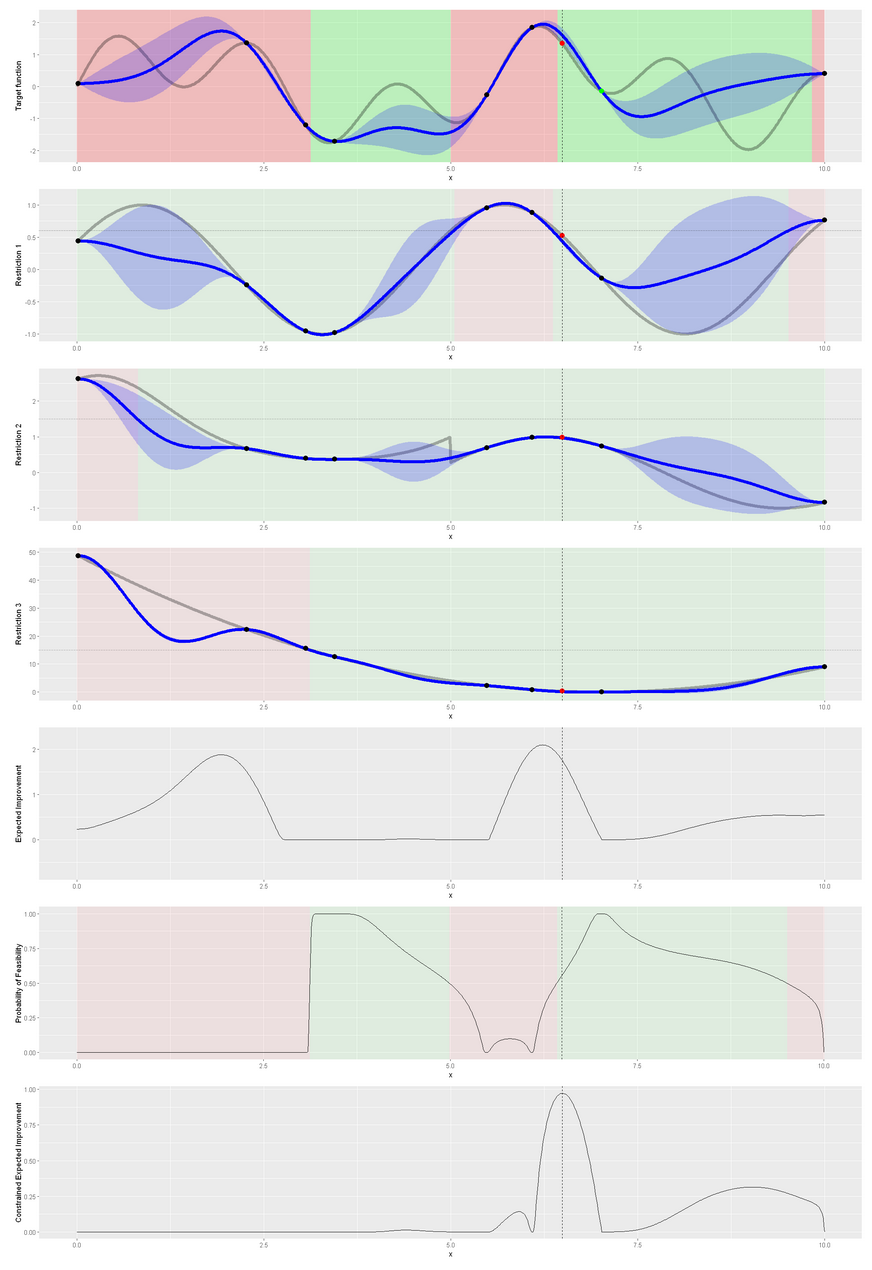
\includegraphics[width=\textwidth]{figures/bo_gp_regression_constraints}
	\decoRule
	\caption[Constrained Bayesian Optimization]{(Constrained) Bayesian Optimization using a Gaussian process after the eighth observed point. The acquisition function used is the Constrained Expected Improvement, combining the Expected Improvement with the probability of feasibility acquisition functions.}
	\label{fig:bo_gp_regression_constraints}
\end{figure}

Other alternative methods exist to incorporate constraints as well [\cite{paulson_cobalt_2021}][\cite{ungredda_bayesian_2021}][\cite{hernandez-lobato_general_2016}][\cite{swiler_survey_2020}][\cite{lam_lookahead_nodate}].

One related subject to constraints is the possibility to place priors on the input values to guide the optimization process [\cite{souza_bayesian_2021}]. Priors do not impose hard restrictions, only a starting hypothesis on the optimal values that gets progressively overshadowed in the presence of more evidence (i.e. data) [\cite{stark_constraints_2015}].

\section{Calibration over original inputs}

In the standard calibration procedure we change the transition probabilities in the matrices, assuming they are independent and enforcing constraints in the error calculation step. One alternative would be to calibrate over those relevant original inputs (i.e. those found in the literature, studies, expert opinions, ...) and then calculate the transition probabilities (and possibly other inputs of the model) from them. With this method we preserve and inject the knowledge we have about the domain into the model (that is, how to calculate the probabilities from the scientific sources, assumptions, implicit restrictions, ...).

\begin{figure}[h]
	\centering
	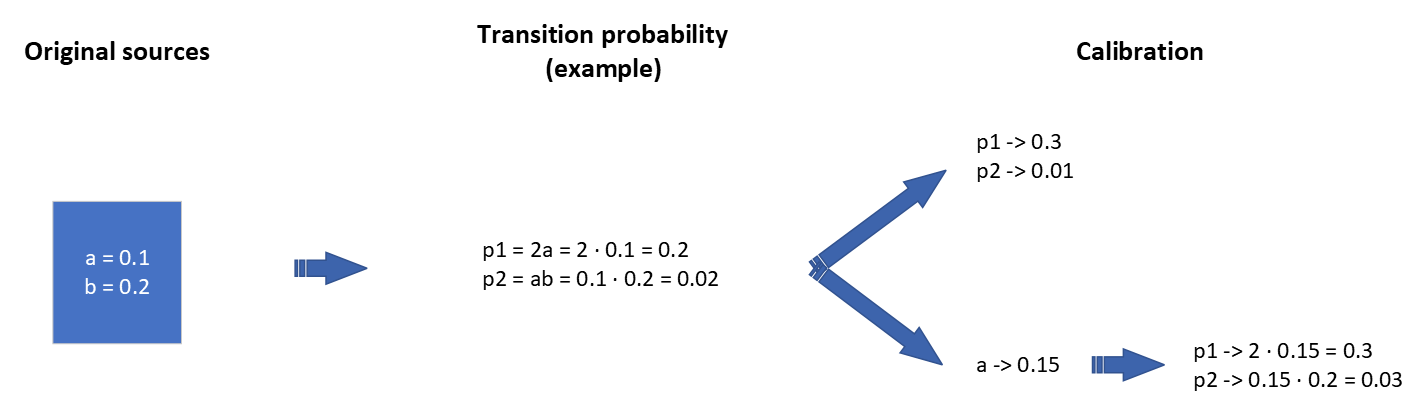
\includegraphics[width=\textwidth]{figures/calibration_inputs}
	\decoRule
	\caption[Calibration over inputs]{Calibration procedures: directly over the probabilities (``Calibration'', top) and over the original inputs (``Calibration'', bottom).}
	\label{fig:calibration_inputs}
\end{figure}

Since we calibrate to account for the uncertainty in the natural history and the probabilities in the matrices are calculated from parameters, we could classify the uncertainty sources in two: uncertainty associated to the inputs and uncertainty associated to the calculation of the probability.

\subsection{Parameter uncertainty}
If we are sure about the calculation of the transition probability, like a well-known relationship (e.g. Bayes formula), the remaining sources of uncertainty are the inputs themselves. In this case we can set up the optimizer to change these inputs, recalculate the probabilities and run the model.

For interpretation and sanity check purposes we can check both the changed input value and the newly-calculated transition probability.

\begin{figure}[h!]
	\centering
	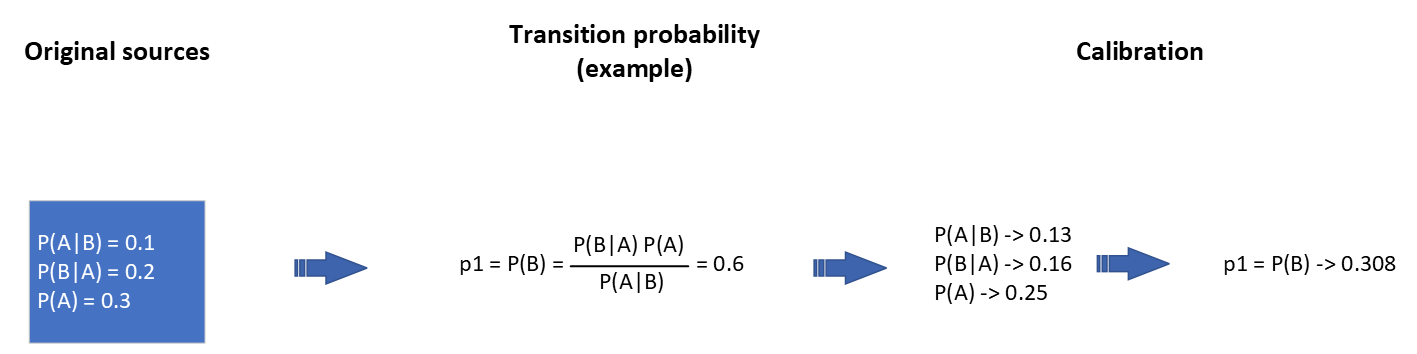
\includegraphics[width=\textwidth]{figures/calibration_values}
	\decoRule
	\caption[Calibration over input values]{If we are certain of the relationship between the probability and the inputs, we can calibrate over the inputs and we will get the calibrated probability by preserving the link with the original inputs.}
	\label{fig:calibration_values}
\end{figure}

\subsection{Calculation uncertainty}
Beyond the inputs, the calculation itself might be uncertain as well, for example by making a very rough approximation or assuming a probabilistic distribution with a poor fit. In this case we can insert an error term or scaling factor in the formula to account for the misspecification, with a neutral initial value (0 if error, 1 if factor). Then, the calibration could include these error/scaling terms in the set of parameters to be optimized.

For interpretation and sanity check purposes, besides the probabilities themselves as usual, we can check the error term/scaling factor. If they are too different from the initial values we might conclude that the calculation is not trustworthy and we might have to review our assumptions. Also, if the calculation is a very rough estimate another alternative would be to reject the calculation itself and optimize the probability value as usual.

\begin{figure}[h!]
	\centering
	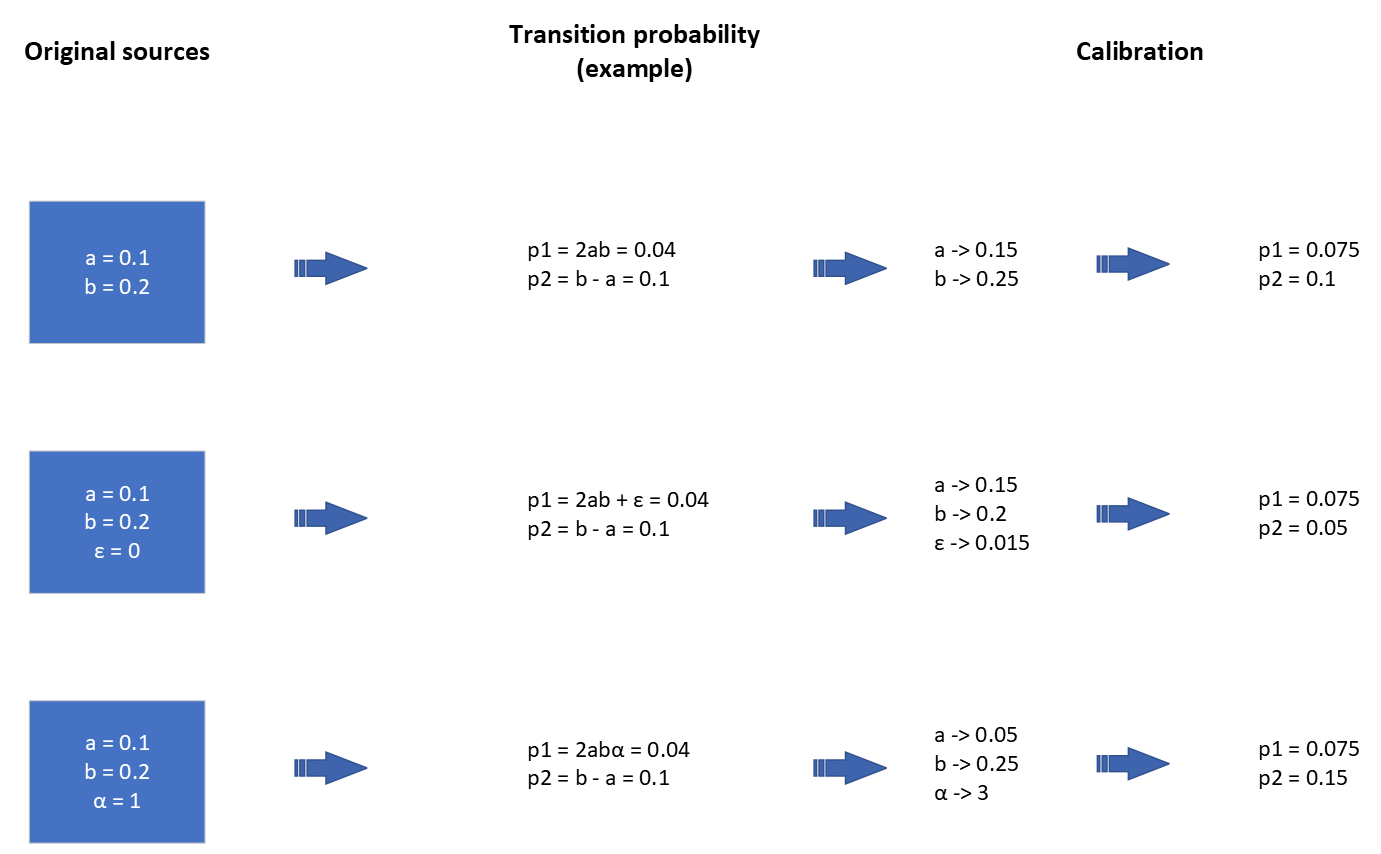
\includegraphics[width=\textwidth]{figures/calibration_calculation}
	\decoRule
	\caption[Calibration over calculations]{To account for the possibility of a misspecified calculation we can add additional terms to a formula. We can see calibration with no formula flexibility (top row), an additive error term for p1 (middle row) or a multiplicative factor for p1 (bottom row).}
	\label{fig:calibration_calculation}
\end{figure}

\subsection{Comments}

\subsubsection*{Pros}
\begin{itemize}
	\item Preserving the link and implicit knowledge between the original sources and the calculated probabilities
	\item Preserving relationships between probabilities and (some kinds of) constraints
\end{itemize}

\subsubsection*{Cons}
\begin{itemize}
	\item Overcomplicating the calibration procedure in simple cases
	\item Relationships might not be too complicated
\end{itemize}

\section{Input/probabilities dependencies using graph theory}

\begin{figure}[h!]
	\centering
	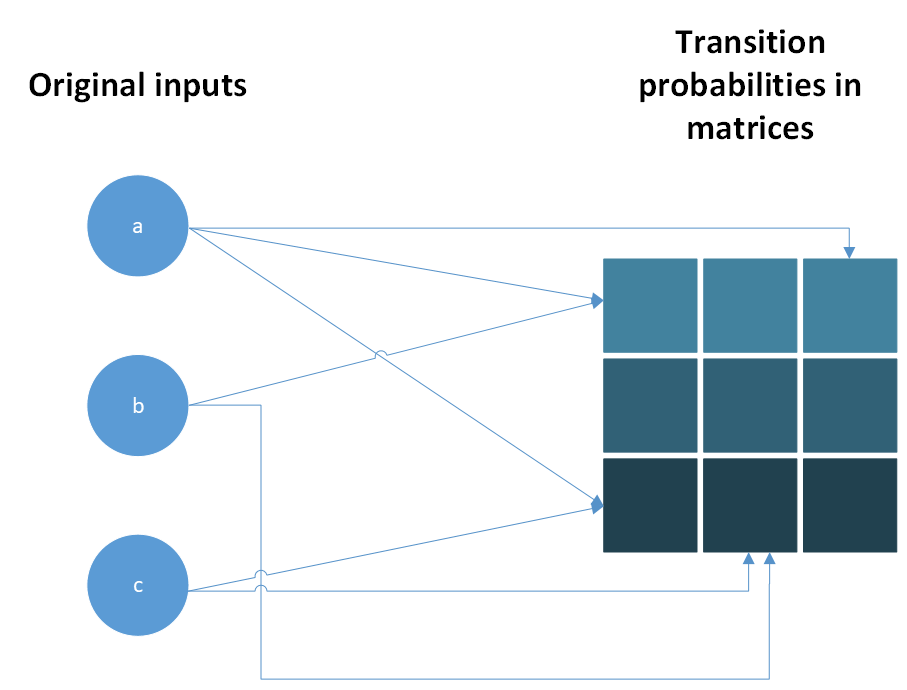
\includegraphics[width=\textwidth]{figures/graph_input_probs}
	\decoRule
	\caption[Dependency graph between inputs and transition probabilities]{We could use graph theory to help optimization considering the dependencies between inputs and the transition probabilities in the matrices.}
	\label{fig:graph_input_probs}
\end{figure}

\subsection{Comments}

\subsubsection*{Pros}
\begin{itemize}
	\item Might help the calibration procedure by exploiting domain knowledge
\end{itemize}

\subsubsection*{Cons}
\begin{itemize}
	\item Overcomplicating the calibration procedure in simple cases
	\item Relationships might not be too complicated
	\item Too vague at this point
\end{itemize}
% Chapter 1
\chapter{Tests performed} % Main chapter title

\label{sec:tests} % For referencing the chapter elsewhere, use \ref{Chapter1} 

\section{Test model: lung cancer}

\begin{itemize}
	\item Total of 9 matrices (one per age group: 35-39, 40-44, …, 75-79).
	\item 7 health states: healthy, stages I-II, stage IIIa, stage IIIb, LC survival, death from LC, death from other causes → 7x7 matrices. Sometimes the LC survival state is excluded from the calibration resulting in 6x6 matrices.
	\item Matrices represent monthly steps in the simulation. Since they are applied for 5-year groups, each matrix is used in 5 * 12 = 60 iterations in the model.
	\item A simplified calibration can be performed without running the model, only the matrices are used. This is a fast approximation since we are not considering some factors of the full model (e.g. prevalence of smoking):
	\begin{itemize}
		\item LC survival state is excluded → 6x6 matrices
		\item From the 6x6=36 probabilities per matrix, only 11 probabilities are allowed to change. The rest are either constant (zeroes, ones) or one minus the sum of the rest of the row.
		\item The error measurement is a weighted sum of the absolute differences of the LC incidence, LC mortality and mortality from other causes. The weights are 0.45, 0.45 and 0.10 respectively.
	\end{itemize}
\end{itemize}

\section{Simplified calibration}
\subsection{1 matrix}

\begin{itemize}
	\item Source file: models/lung/calibration\_wrapper.R (N\_MATRICES set to 1)
	\item Only the first age group is being calibrated (35-39): 1x11 = 11 parameters.
\end{itemize}

\begin{table}[h]
	\begin{tabular}{p{2cm}|l|l|l|l}
		\textbf{Algorithm} 		& \textbf{Initial matrix} & \textbf{Nelder-Mead} 		& \textbf{Particle swarm} 	& \textbf{Bayesian} \\
		\hline \\
		\textbf{Error}	& 1.1545799674960& 0.6633085653748	& \cellcolor{green}0.66298515		& \cellcolor{green}0.6629851533965 \\
		\textbf{Time (s)} & - & \cellcolor{green}0.76 & 22.97 & \cellcolor{red!20}114.89 \\
		\textbf{Evaluations} & - & 252 & \cellcolor{red!20}10100 & \cellcolor{green}21 \\
	\end{tabular}
\end{table}

\subsection{2 matrices}

\begin{itemize}
	\item Source file: models/lung/calibration\_wrapper.R (N\_MATRICES set to 2)
	\item The first and second age groups are being calibrated (35-39 and 40-44): 2x11 = 22 parameters.
\end{itemize}


\begin{table}[h]
	\begin{tabular}{p{2cm}|l|l|l|l}
		\textbf{Algorithm} 		& \textbf{Initial matrix} & \textbf{Nelder-Mead} 		& \textbf{Particle swarm} 	& \textbf{Bayesian} \\
		\hline \\
		\textbf{Error}	& 1.6495138536869 & 0.7333381543348456 & \cellcolor{green}0.72801101 & \cellcolor{green}0.7287116136105645 \\
		\textbf{Time (s)} & - & \cellcolor{green}4.44 & 24.46 & \cellcolor{red!20}421.69 \\
		\textbf{Evaluations} & - & 2092 & \cellcolor{green}10100 & \cellcolor{green}70 \\
	\end{tabular}
\end{table}

\subsection{All (9) matrices}

\begin{itemize}
    \item Source file: models/lung/calibration\_wrapper.R (N\_MATRICES set to 9)
	\item All age groups are being calibrated: 9x11 = 99 parameters.
	\item Standard bayesian optimization takes too much time and the process was aborted before completion. Other strategies could be attempted: calibrate matrices sequentially, restrict number of parameters, optimize gaussian process regression (see section \ref{sec:proposal}), ...
\end{itemize}

\begin{table}[h]
	\begin{tabular}{p{2cm}|l|l|l|l}
		\textbf{Algorithm} 		& \textbf{Initial matrix} & \textbf{Nelder-Mead} 		& \textbf{Particle swarm} 	& \textbf{Bayesian} \\
		\hline \\
		\textbf{Error}	& 6.6842251473203 & 4.0210661197016	& 4.3594607 & \cellcolor{red}6.142333876 \\
		\textbf{Time (s)} & - & 57.58 & 35.64 & \cellcolor{red}31352 \\
		\textbf{Evaluations} & - & 19800 & 9407 & \cellcolor{red}50 \\
	\end{tabular}
\end{table}

\subsection{Method comparison}

\begin{figure}[!htb]
	\centering
	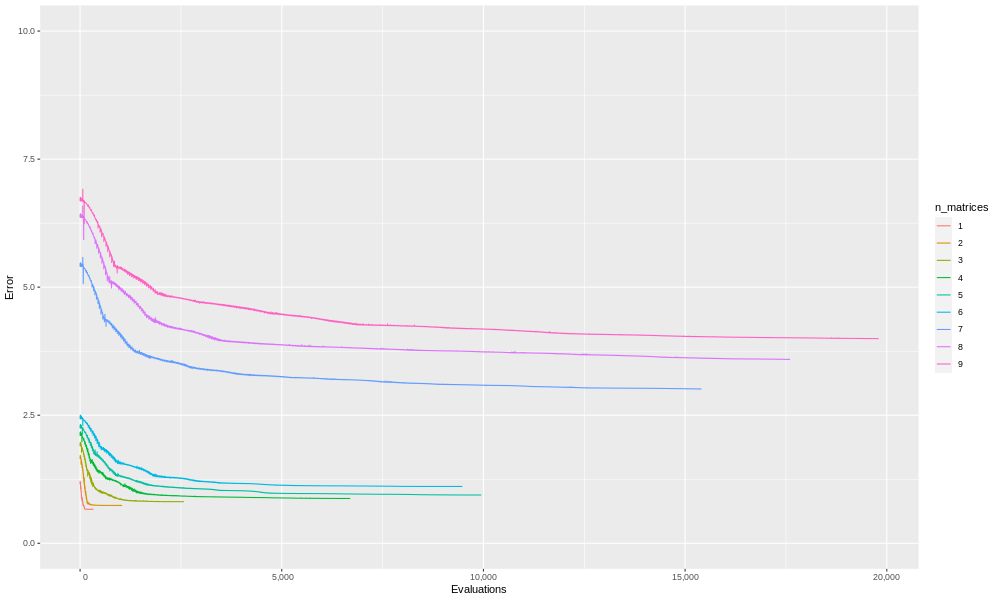
\includegraphics[width=\textwidth]{figures/alg_nelder-mead}
	\decoRule
	\caption[Nelder-Mead]{Nelder-Mead error by iteration step}
	\label{fig:alg_nelder-mead}
\end{figure}

\begin{figure}[!htb]
\centering
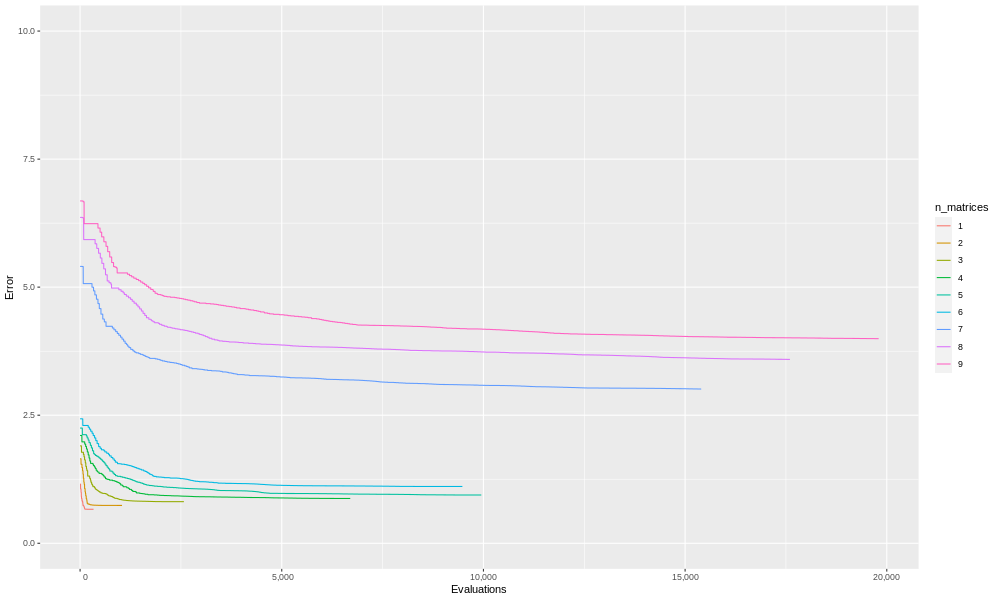
\includegraphics[width=\textwidth]{figures/alg_nelder-mead_smoothed}
\decoRule
\caption[Nelder-Mead (smoothed)]{Nelder-Mead smoothed error by iteration step (cumulative minimum)}
\label{fig:alg_nelder-mead_smoothed}
\end{figure}

\begin{figure}[!htb]
\centering
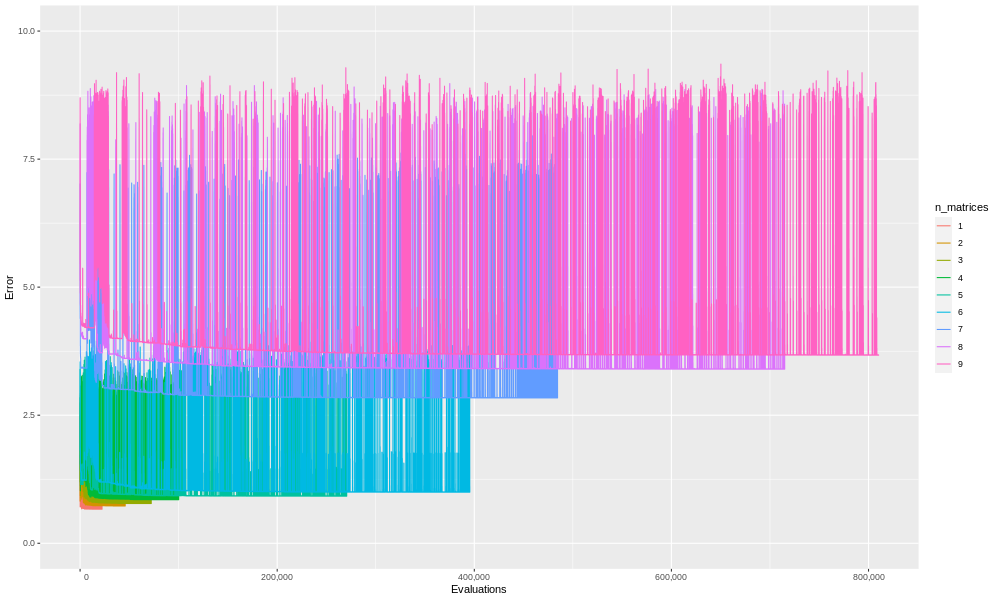
\includegraphics[width=\textwidth]{figures/alg_annealing}
\decoRule
\caption[Simulated Annealing]{Simulated Annealing error by iteration step}
\label{fig:alg_annealing}
\end{figure}

\begin{figure}[!htb]
\centering
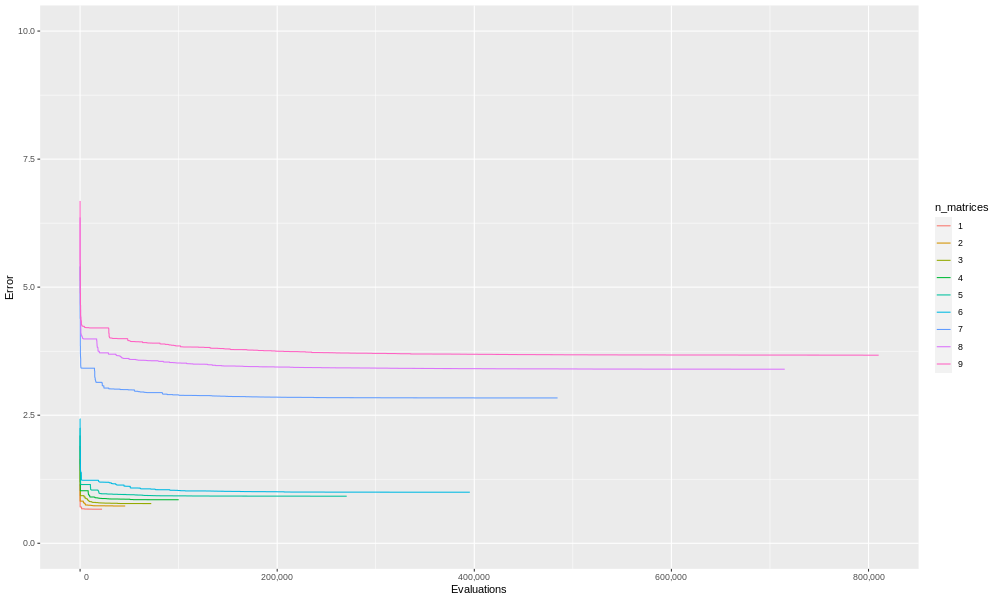
\includegraphics[width=\textwidth]{figures/alg_annealing_smoothed}
\decoRule
\caption[Simulated Annealing (smoothed)]{Simulated Annealing smoothed error by iteration step (cumulative minimum)}
\label{fig:alg_annealing_smoothed}
\end{figure}

\begin{figure}[!htb]
\centering
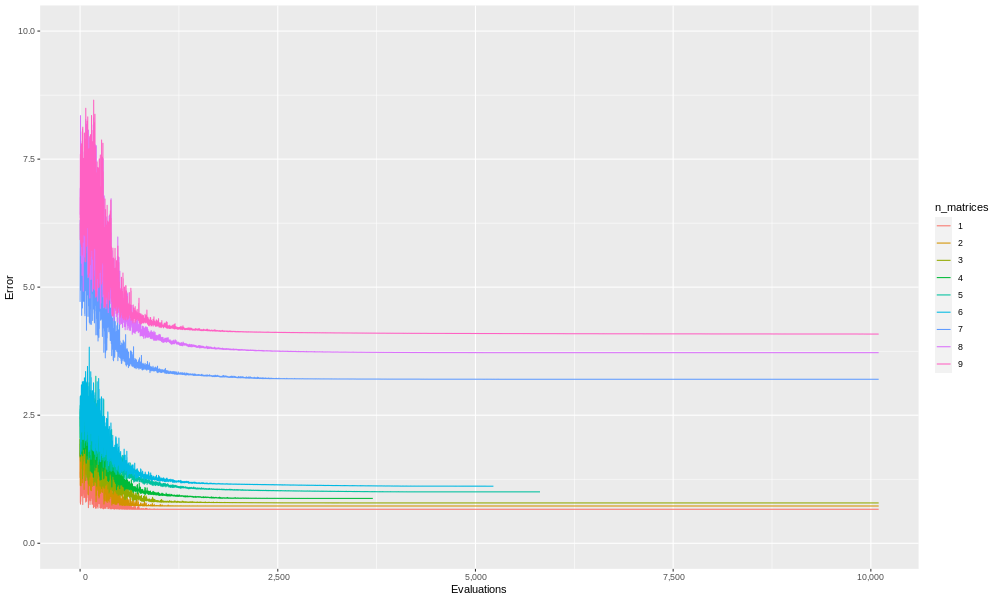
\includegraphics[width=\textwidth]{figures/alg_pso}
\decoRule
\caption[Particle Swarm Optimization]{Particle Swarm Optimization error by iteration step}
\label{fig:alg_pso}
\end{figure}

\begin{figure}[!htb]
\centering
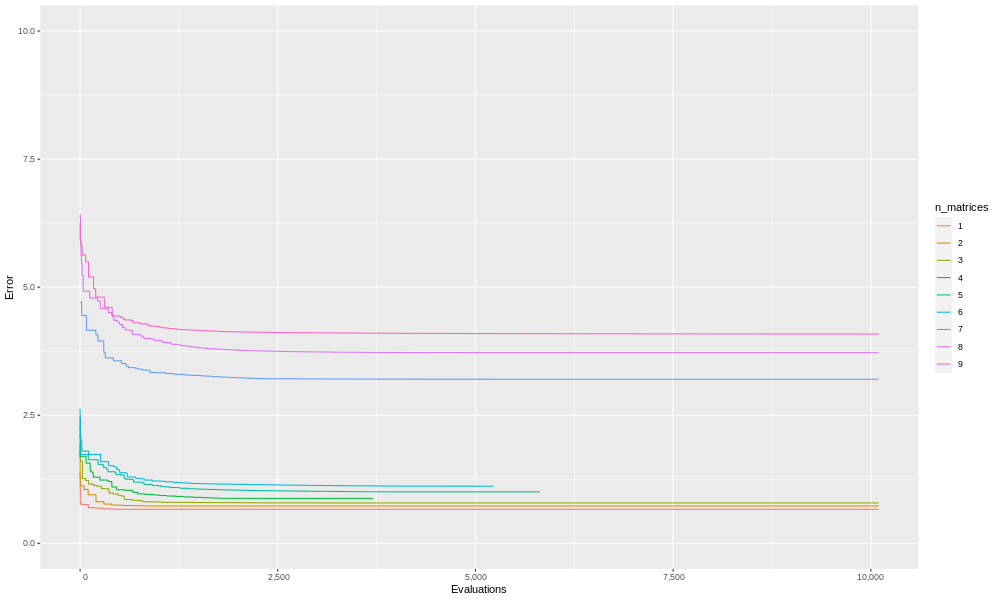
\includegraphics[width=\textwidth]{figures/alg_pso_smoothed}
\decoRule
\caption[Particle Swarm Optimization (smoothed)]{Particle Swarm Optimization smoothed error by iteration step (cumulative minimum)}
\label{fig:alg_pso_smoothed}
\end{figure}

\begin{figure}[!htb]
\centering
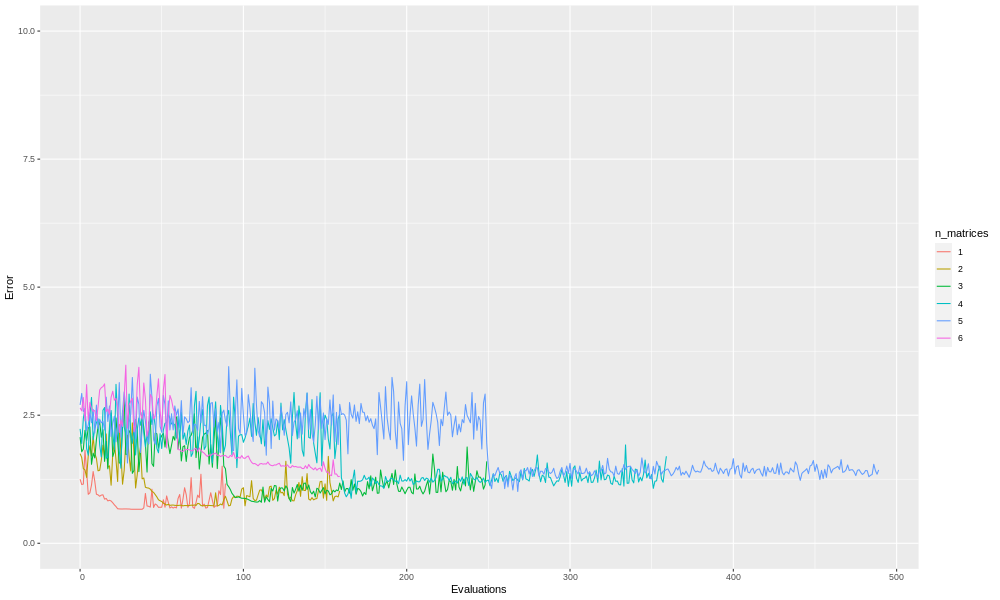
\includegraphics[width=\textwidth]{figures/alg_bayesian}
\decoRule
\caption[Bayesian Optimization]{Bayesian Optimization error by iteration step}
\label{fig:alg_bayesian}
\end{figure}

\begin{figure}[!htb]
\centering
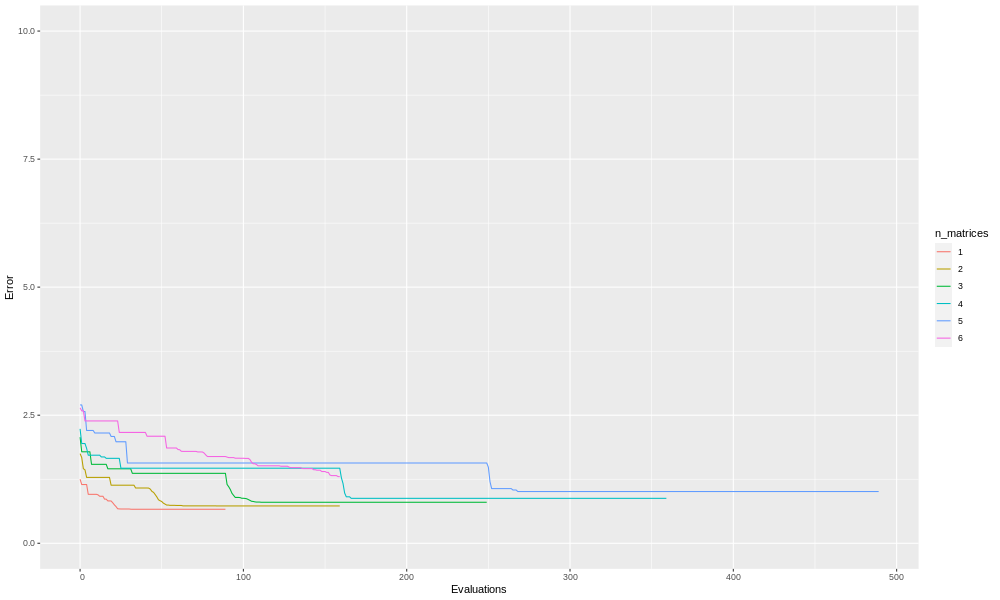
\includegraphics[width=\textwidth]{figures/alg_bayesian_smoothed}
\decoRule
\caption[Bayesian Optimization (smoothed)]{Bayesian Optimization smoothed error by iteration step (cumulative minimum)}
\label{fig:alg_bayesian_smoothed}
\end{figure}


\subsection{Dimensionality comparison}

\begin{figure}[!htb]
	\centering
	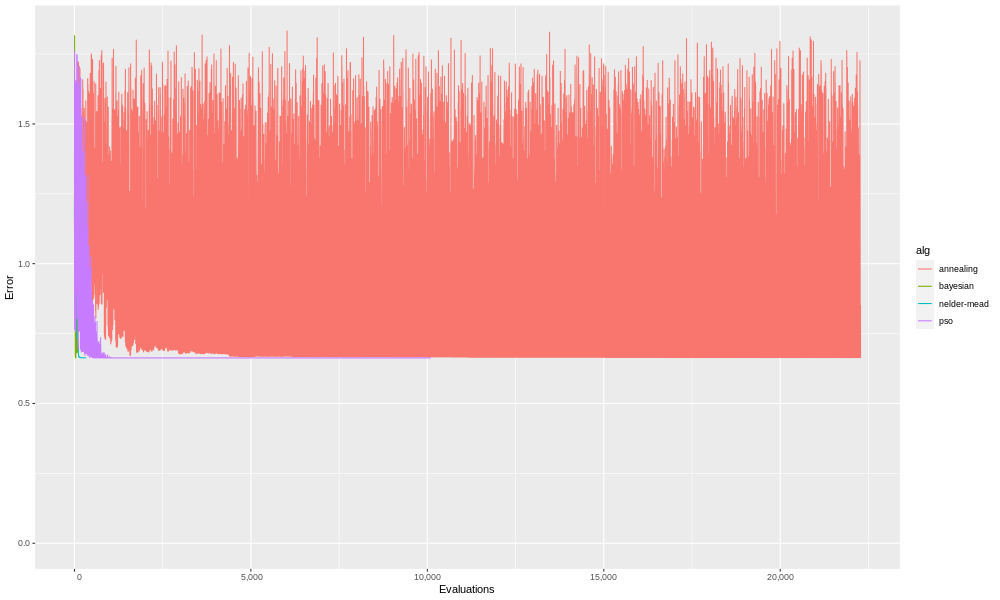
\includegraphics[width=\textwidth]{figures/n_1}
	\decoRule
	\caption[n=1]{Errors on n\_matrices = 1 by method}
	\label{fig:n_1}
\end{figure}

\begin{figure}[!htb]
	\centering
	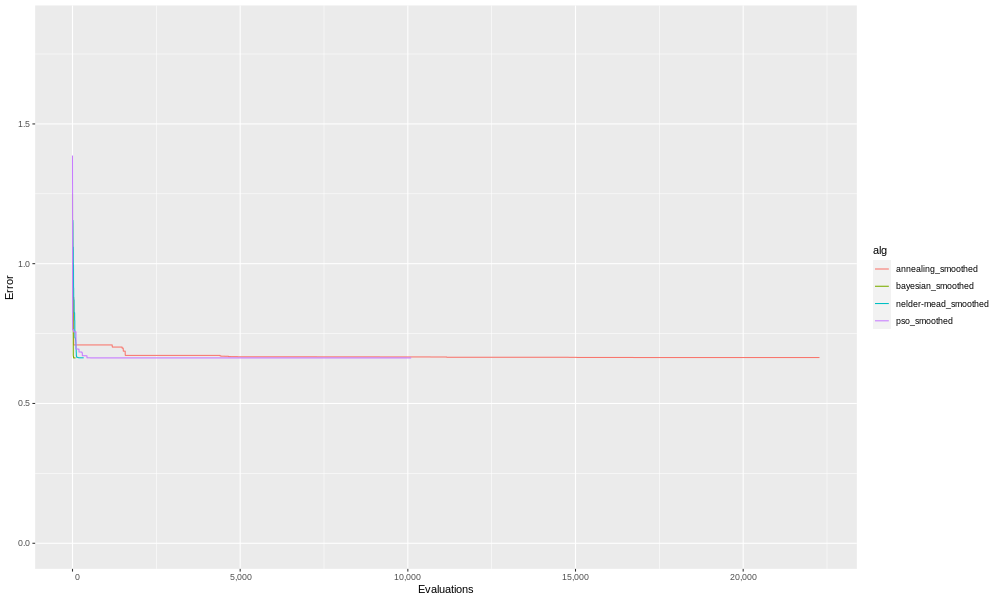
\includegraphics[width=\textwidth]{figures/n_1_smoothed}
	\decoRule
	\caption[n=1 (smoothed)]{(Smoothed) errors on n\_matrices = 1 by method}
	\label{fig:n_1_smoothed}
\end{figure}

\begin{figure}[!htb]
\centering
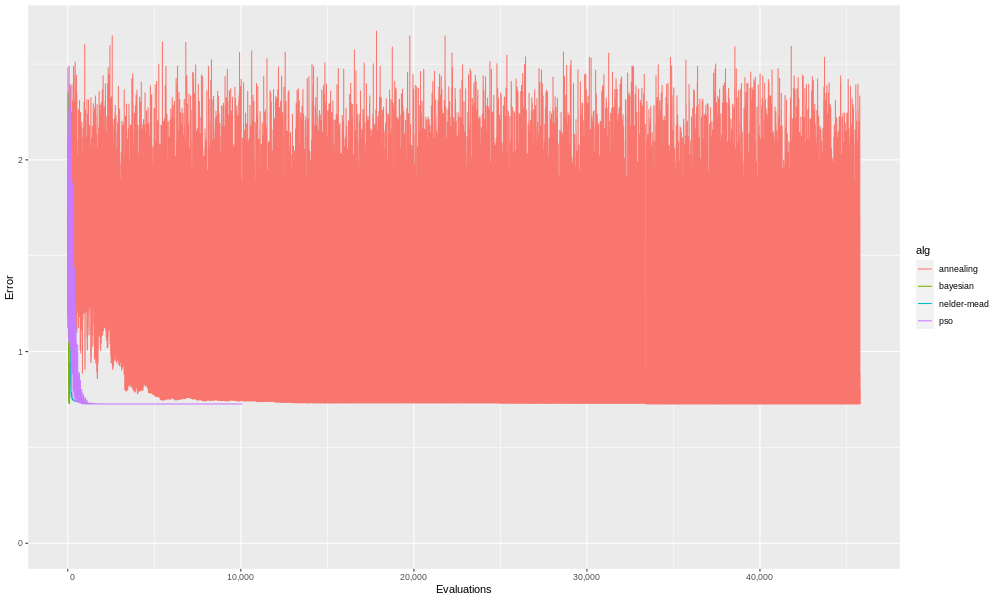
\includegraphics[width=\textwidth]{figures/n_2}
\decoRule
\caption[n=2]{Errors on n\_matrices = 2 by method}
\label{fig:n_2}
\end{figure}

\begin{figure}[!htb]
\centering
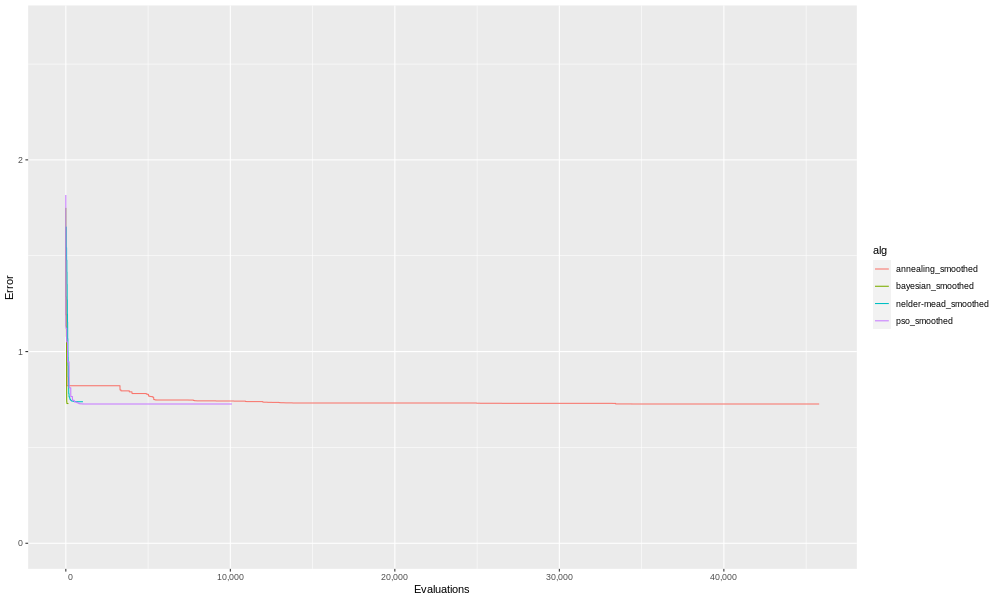
\includegraphics[width=\textwidth]{figures/n_2_smoothed}
\decoRule
\caption[n=2 (smoothed)]{(Smoothed) errors on n\_matrices = 2 by method}
\label{fig:n_2_smoothed}
\end{figure}

\begin{figure}[!htb]
\centering
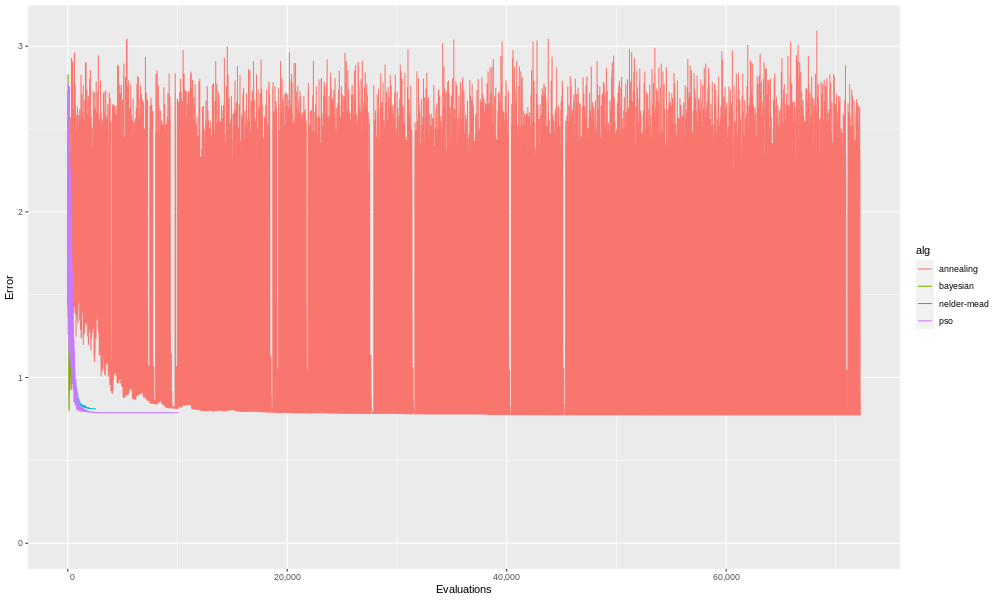
\includegraphics[width=\textwidth]{figures/n_3}
\decoRule
\caption[n=3]{Errors on n\_matrices = 3 by method}
\label{fig:n_3}
\end{figure}

\begin{figure}[!htb]
\centering
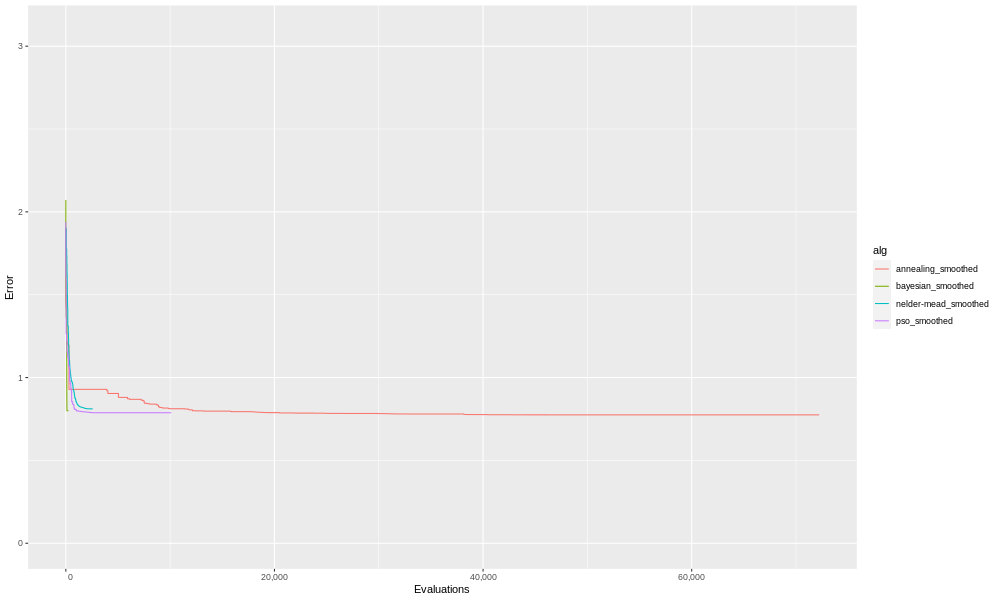
\includegraphics[width=\textwidth]{figures/n_3_smoothed}
\decoRule
\caption[n=3 (smoothed)]{(Smoothed) errors on n\_matrices = 3 by method}
\label{fig:n_3_smoothed}
\end{figure}

\begin{figure}[!htb]
\centering
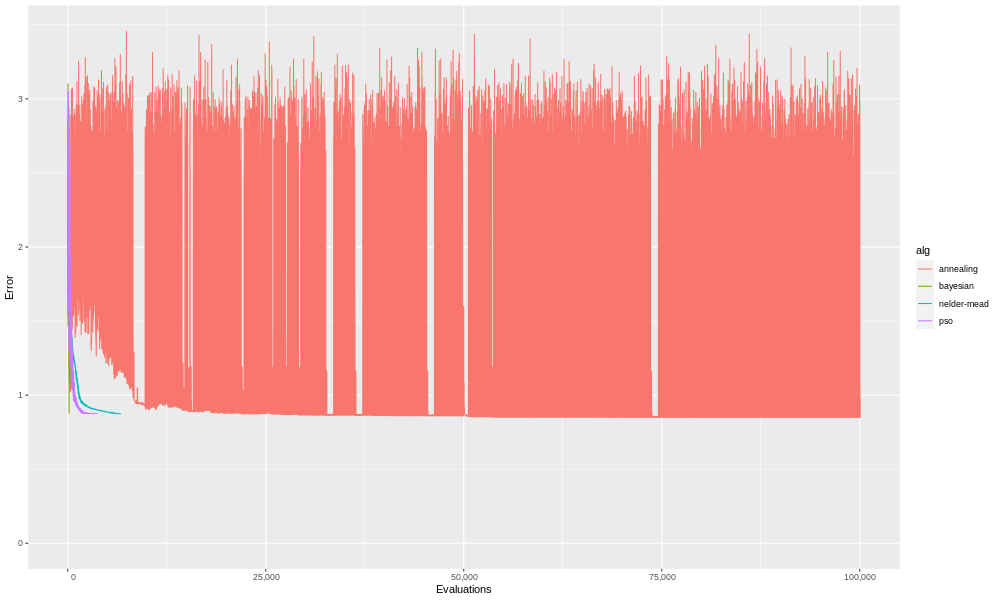
\includegraphics[width=\textwidth]{figures/n_4}
\decoRule
\caption[n=4]{Errors on n\_matrices = 4 by method}
\label{fig:n_4}
\end{figure}

\begin{figure}[!htb]
\centering
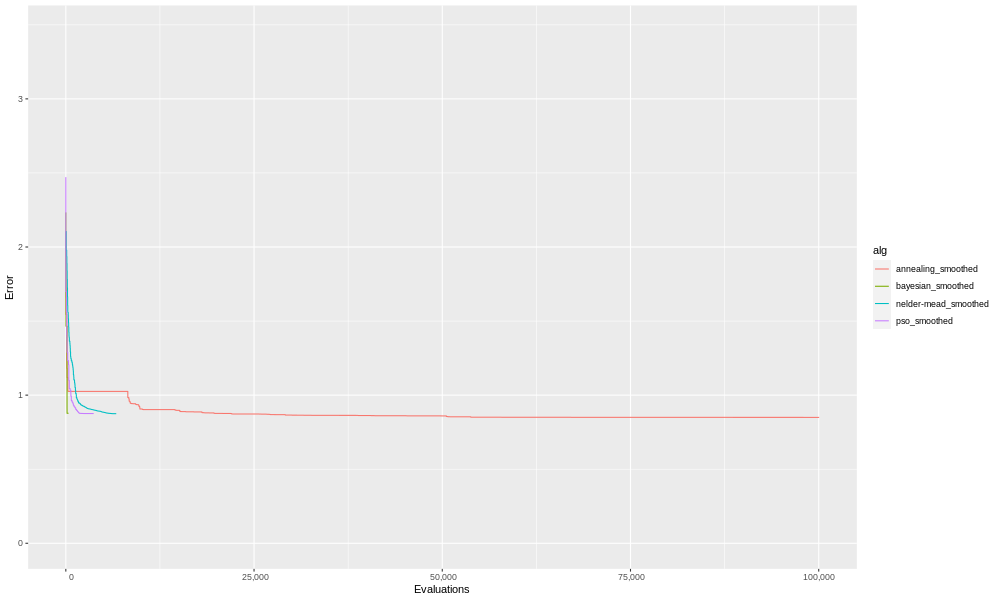
\includegraphics[width=\textwidth]{figures/n_4_smoothed}
\decoRule
\caption[n=4 (smoothed)]{(Smoothed) errors on n\_matrices = 4 by method}
\label{fig:n_4_smoothed}
\end{figure}

\begin{figure}[!htb]
\centering
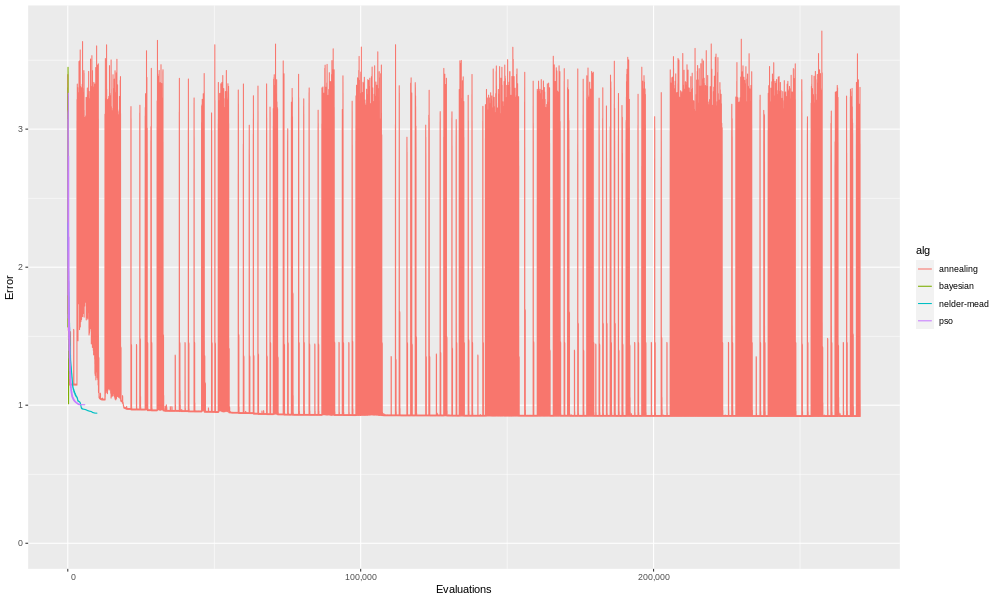
\includegraphics[width=\textwidth]{figures/n_5}
\decoRule
\caption[n=5]{Errors on n\_matrices = 5 by method}
\label{fig:n_5}
\end{figure}

\begin{figure}[!htb]
\centering
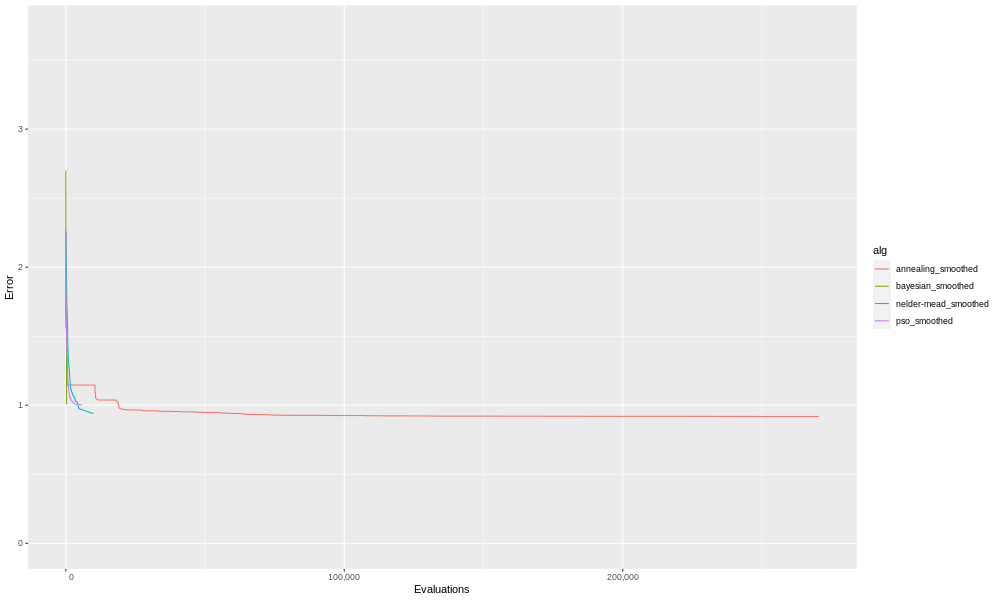
\includegraphics[width=\textwidth]{figures/n_5_smoothed}
\decoRule
\caption[n=5 (smoothed)]{(Smoothed) errors on n\_matrices = 5 by method}
\label{fig:n_5_smoothed}
\end{figure}

\begin{figure}[!htb]
\centering
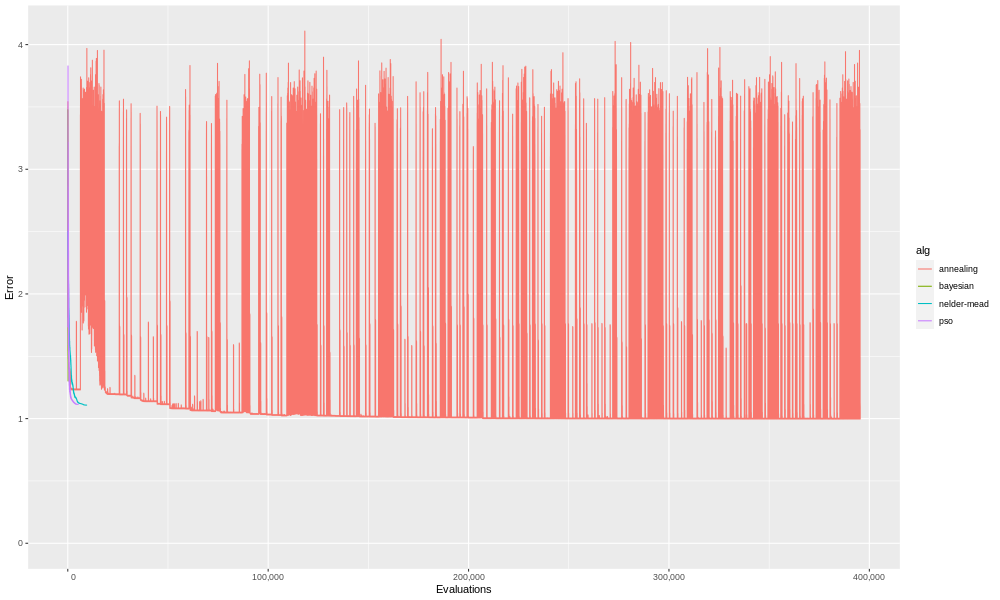
\includegraphics[width=\textwidth]{figures/n_6}
\decoRule
\caption[n=6]{Errors on n\_matrices = 6 by method}
\label{fig:n_6}
\end{figure}

\begin{figure}[!htb]
\centering
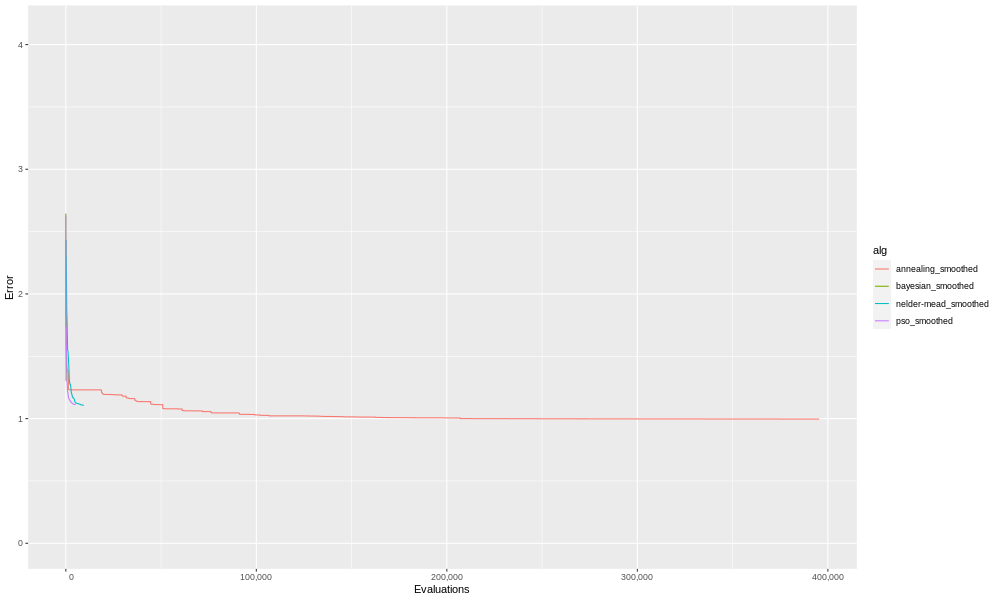
\includegraphics[width=\textwidth]{figures/n_6_smoothed}
\decoRule
\caption[n=6 (smoothed)]{(Smoothed) errors on n\_matrices = 6 by method}
\label{fig:n_6_smoothed}
\end{figure}

\begin{figure}[!htb]
\centering
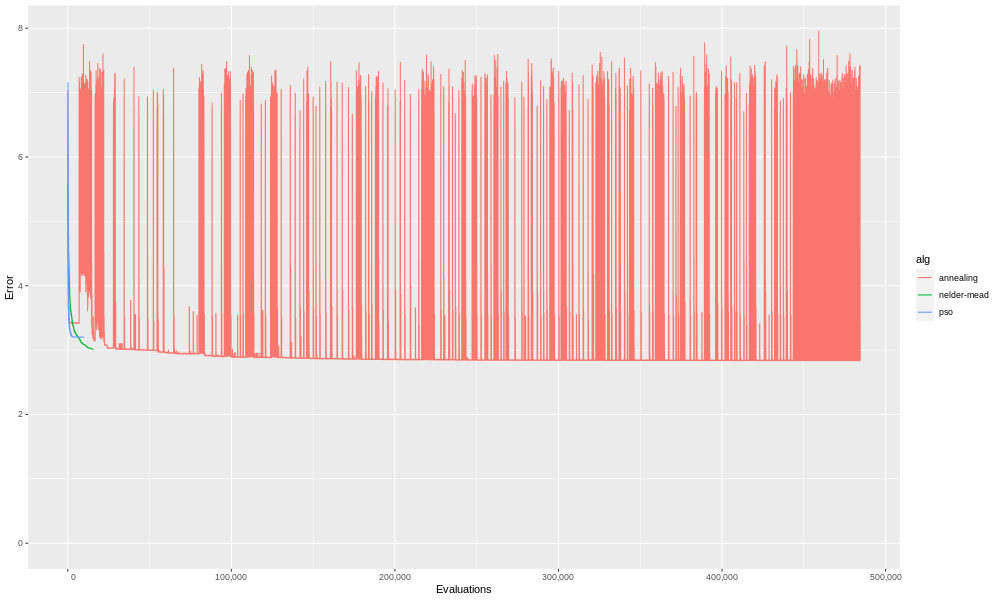
\includegraphics[width=\textwidth]{figures/n_7}
\decoRule
\caption[n=7]{Errors on n\_matrices = 7 by method}
\label{fig:n_7}
\end{figure}

\begin{figure}[!htb]
\centering
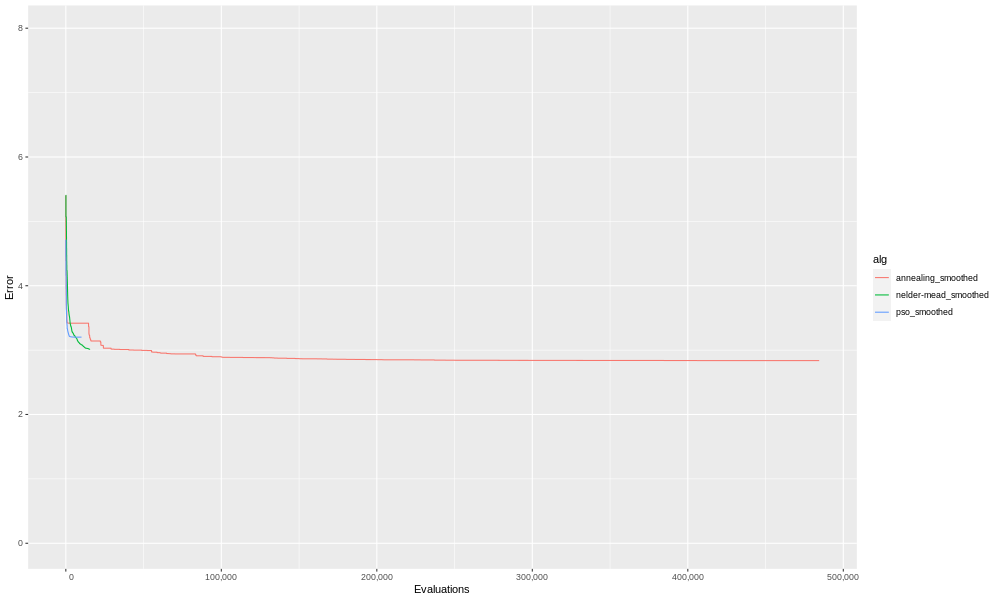
\includegraphics[width=\textwidth]{figures/n_7_smoothed}
\decoRule
\caption[n=7 (smoothed)]{(Smoothed) errors on n\_matrices = 7 by method}
\label{fig:n_7_smoothed}
\end{figure}

\begin{figure}[!htb]
\centering
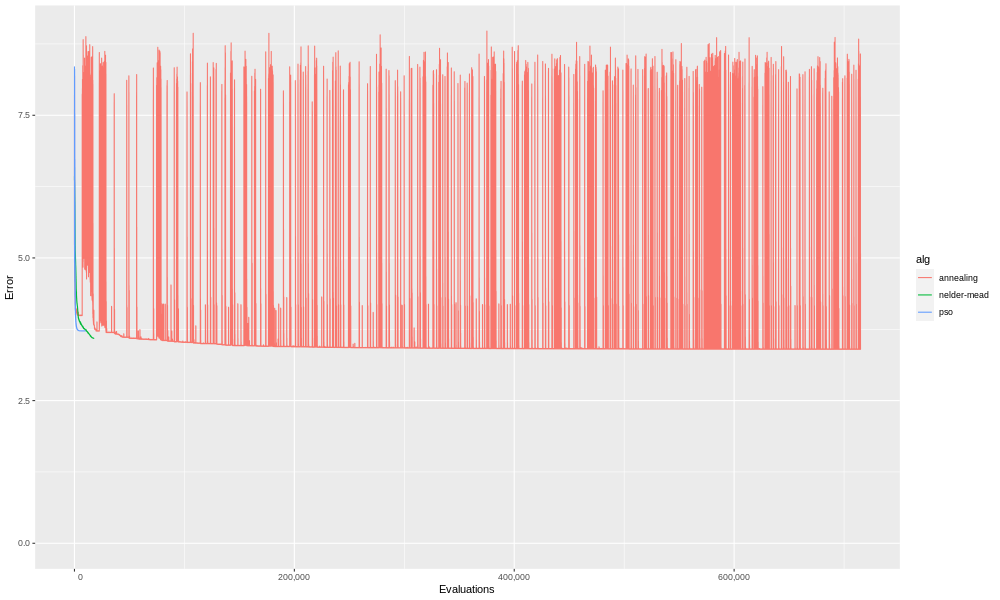
\includegraphics[width=\textwidth]{figures/n_8}
\decoRule
\caption[n=8]{Errors on n\_matrices = 8 by method}
\label{fig:n_8}
\end{figure}

\begin{figure}[!htb]
\centering
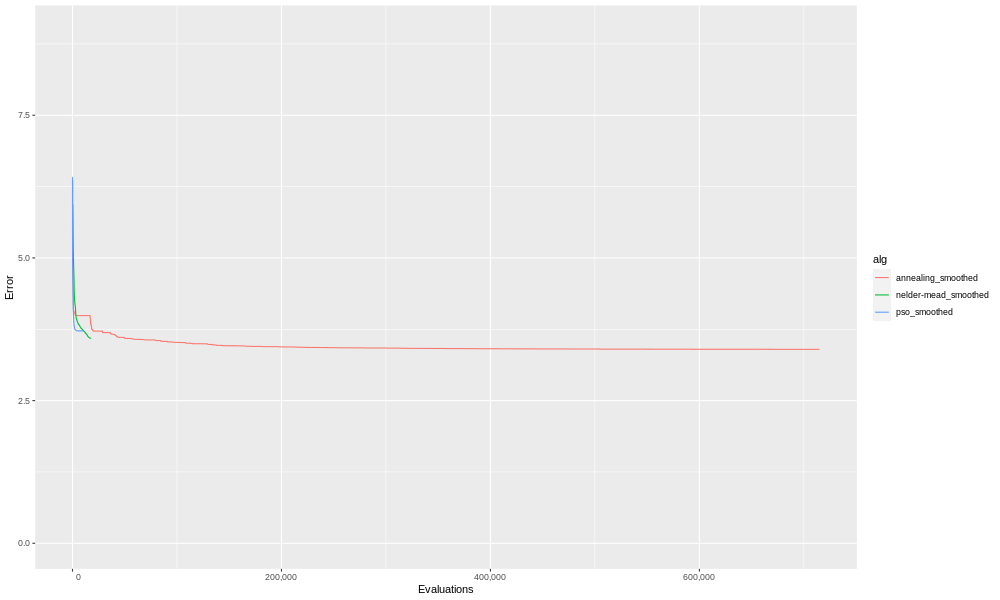
\includegraphics[width=\textwidth]{figures/n_8_smoothed}
\decoRule
\caption[n=8 (smoothed)]{(Smoothed) errors on n\_matrices = 8 by method}
\label{fig:n_8_smoothed}
\end{figure}

\begin{figure}[!htb]
\centering
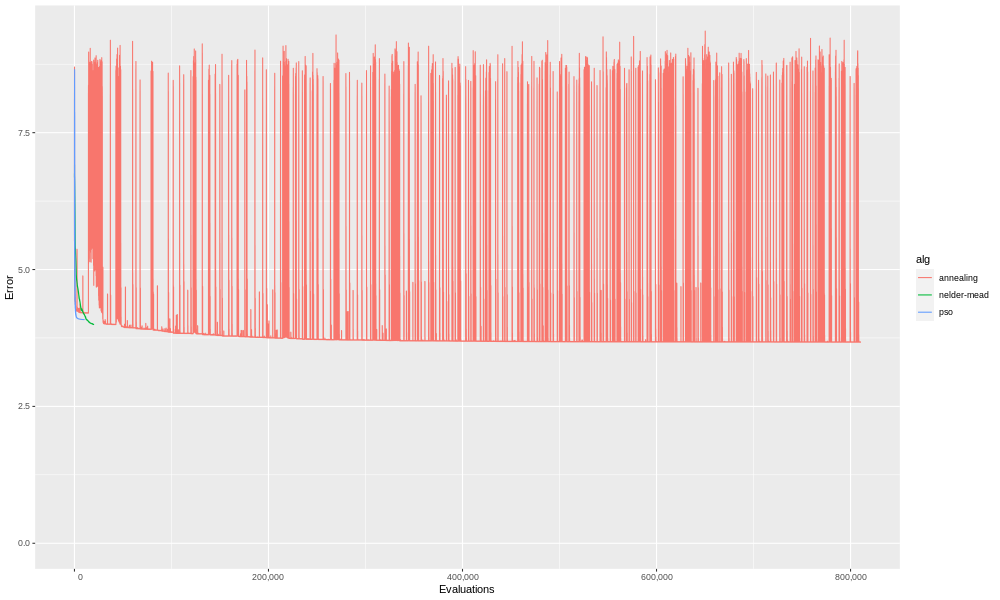
\includegraphics[width=\textwidth]{figures/n_9}
\decoRule
\caption[n=9]{Errors on n\_matrices = 9 by method}
\label{fig:n_9}
\end{figure}

\begin{figure}[!htb]
\centering
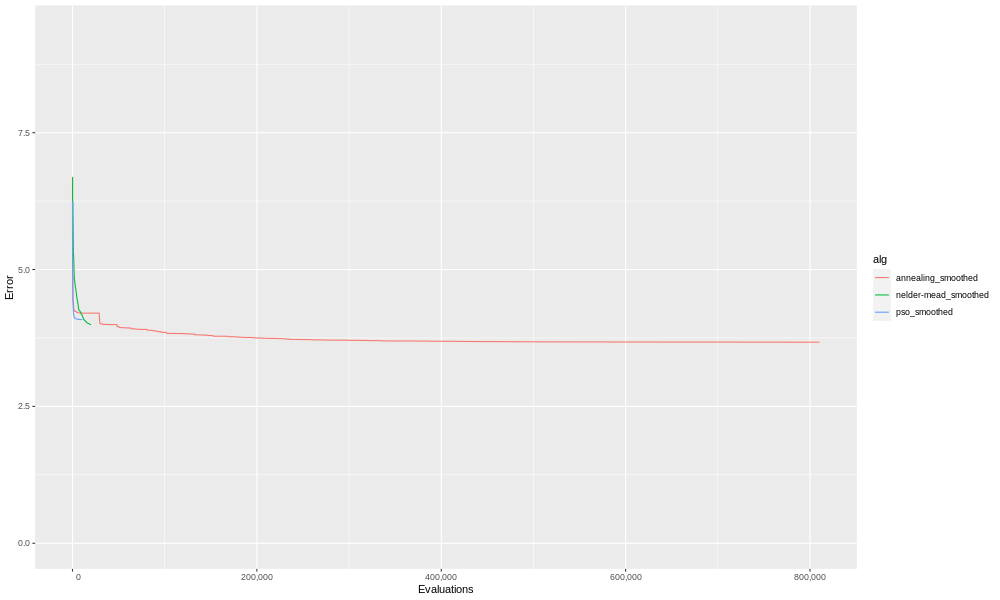
\includegraphics[width=\textwidth]{figures/n_9_smoothed}
\decoRule
\caption[n=9 (smoothed)]{(Smoothed) errors on n\_matrices = 9 by method}
\label{fig:n_9_smoothed}
\end{figure}



\section{Bayesian Optimization (BO) tests}

\begin{figure}[h!]
	\centering
	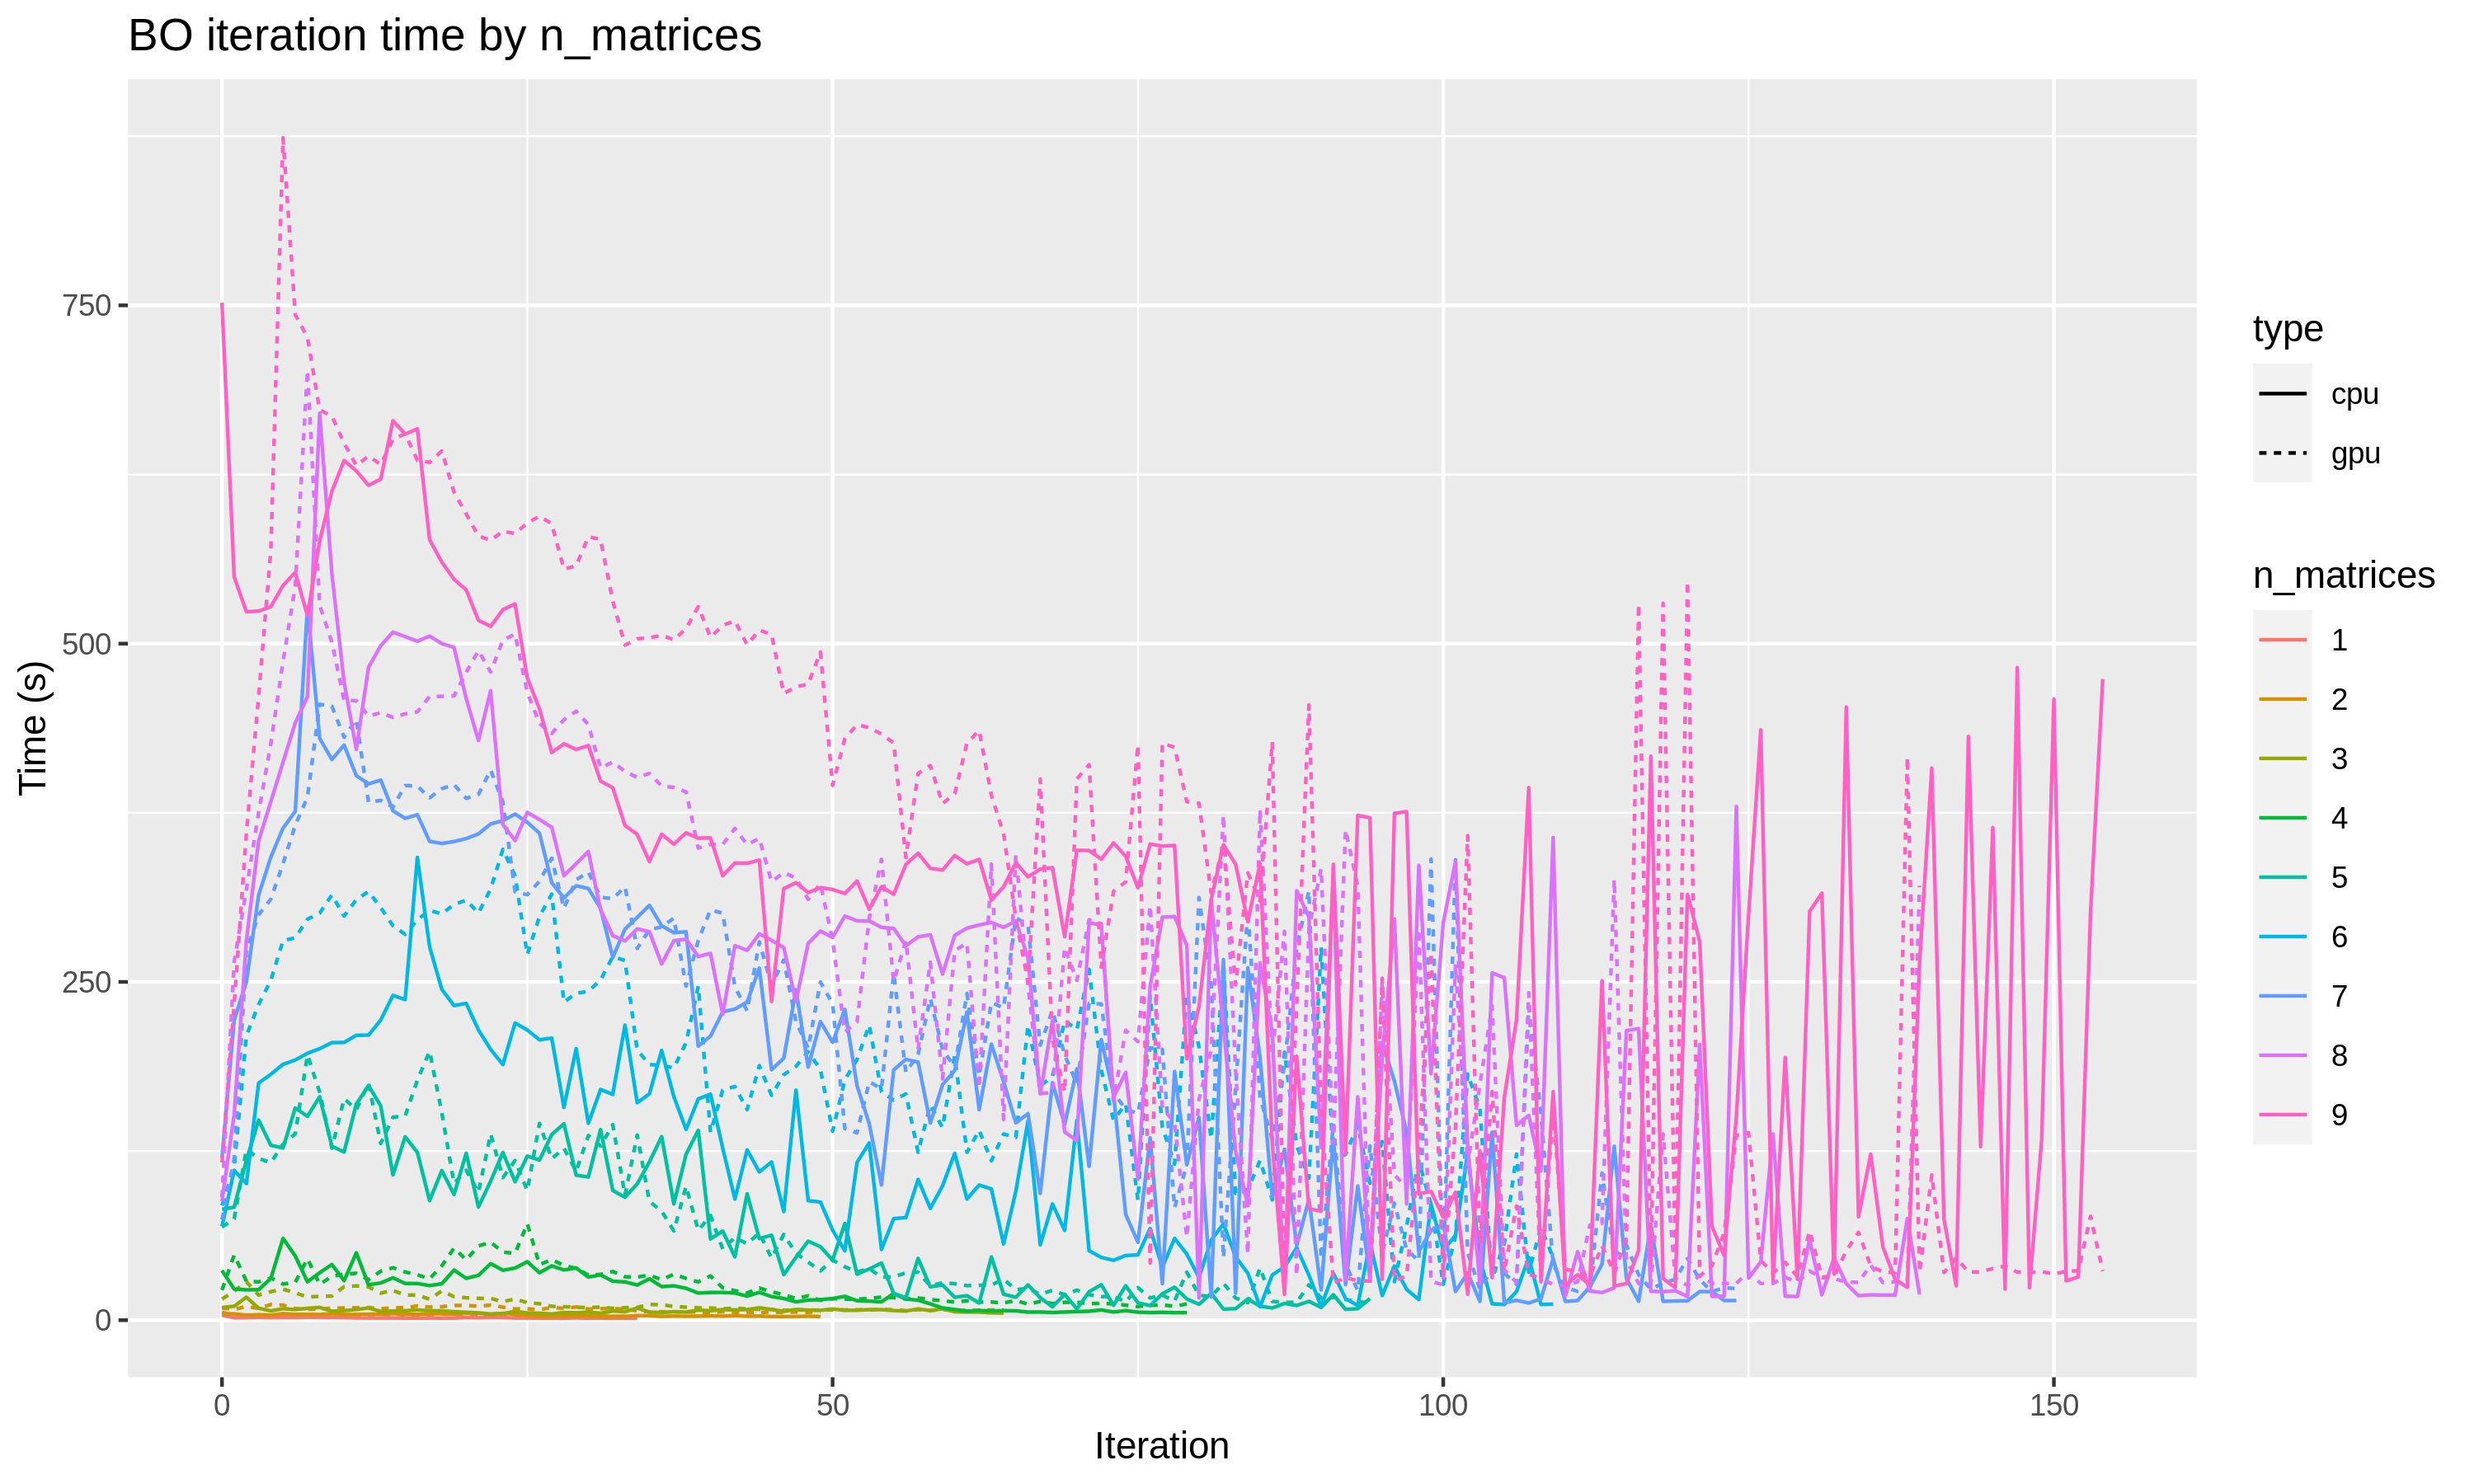
\includegraphics[width=\textwidth]{figures/bo_time}
	\decoRule
	\caption[BO iteration time]{BO iteration time. It increases when the dimensionality increases (different colors) but surprisingly the first iterations take more time than the latter ones, where the opposite is expected. This is a transitory effect as can be seen in figure \ref{fig:bo_time_cpu_long}, using a larger number of iterations. Another surprising outcome is the GPU computation (using a NVIDIA Quadro P620) takes more time than the CPU, but figure \ref{fig:bo_boxplot} shows that the differences are not likely to be significant in the long run. With a powerful GPU this result is expected to change.}
	\label{fig:bo_time}
\end{figure}

\begin{figure}[h!]
\centering
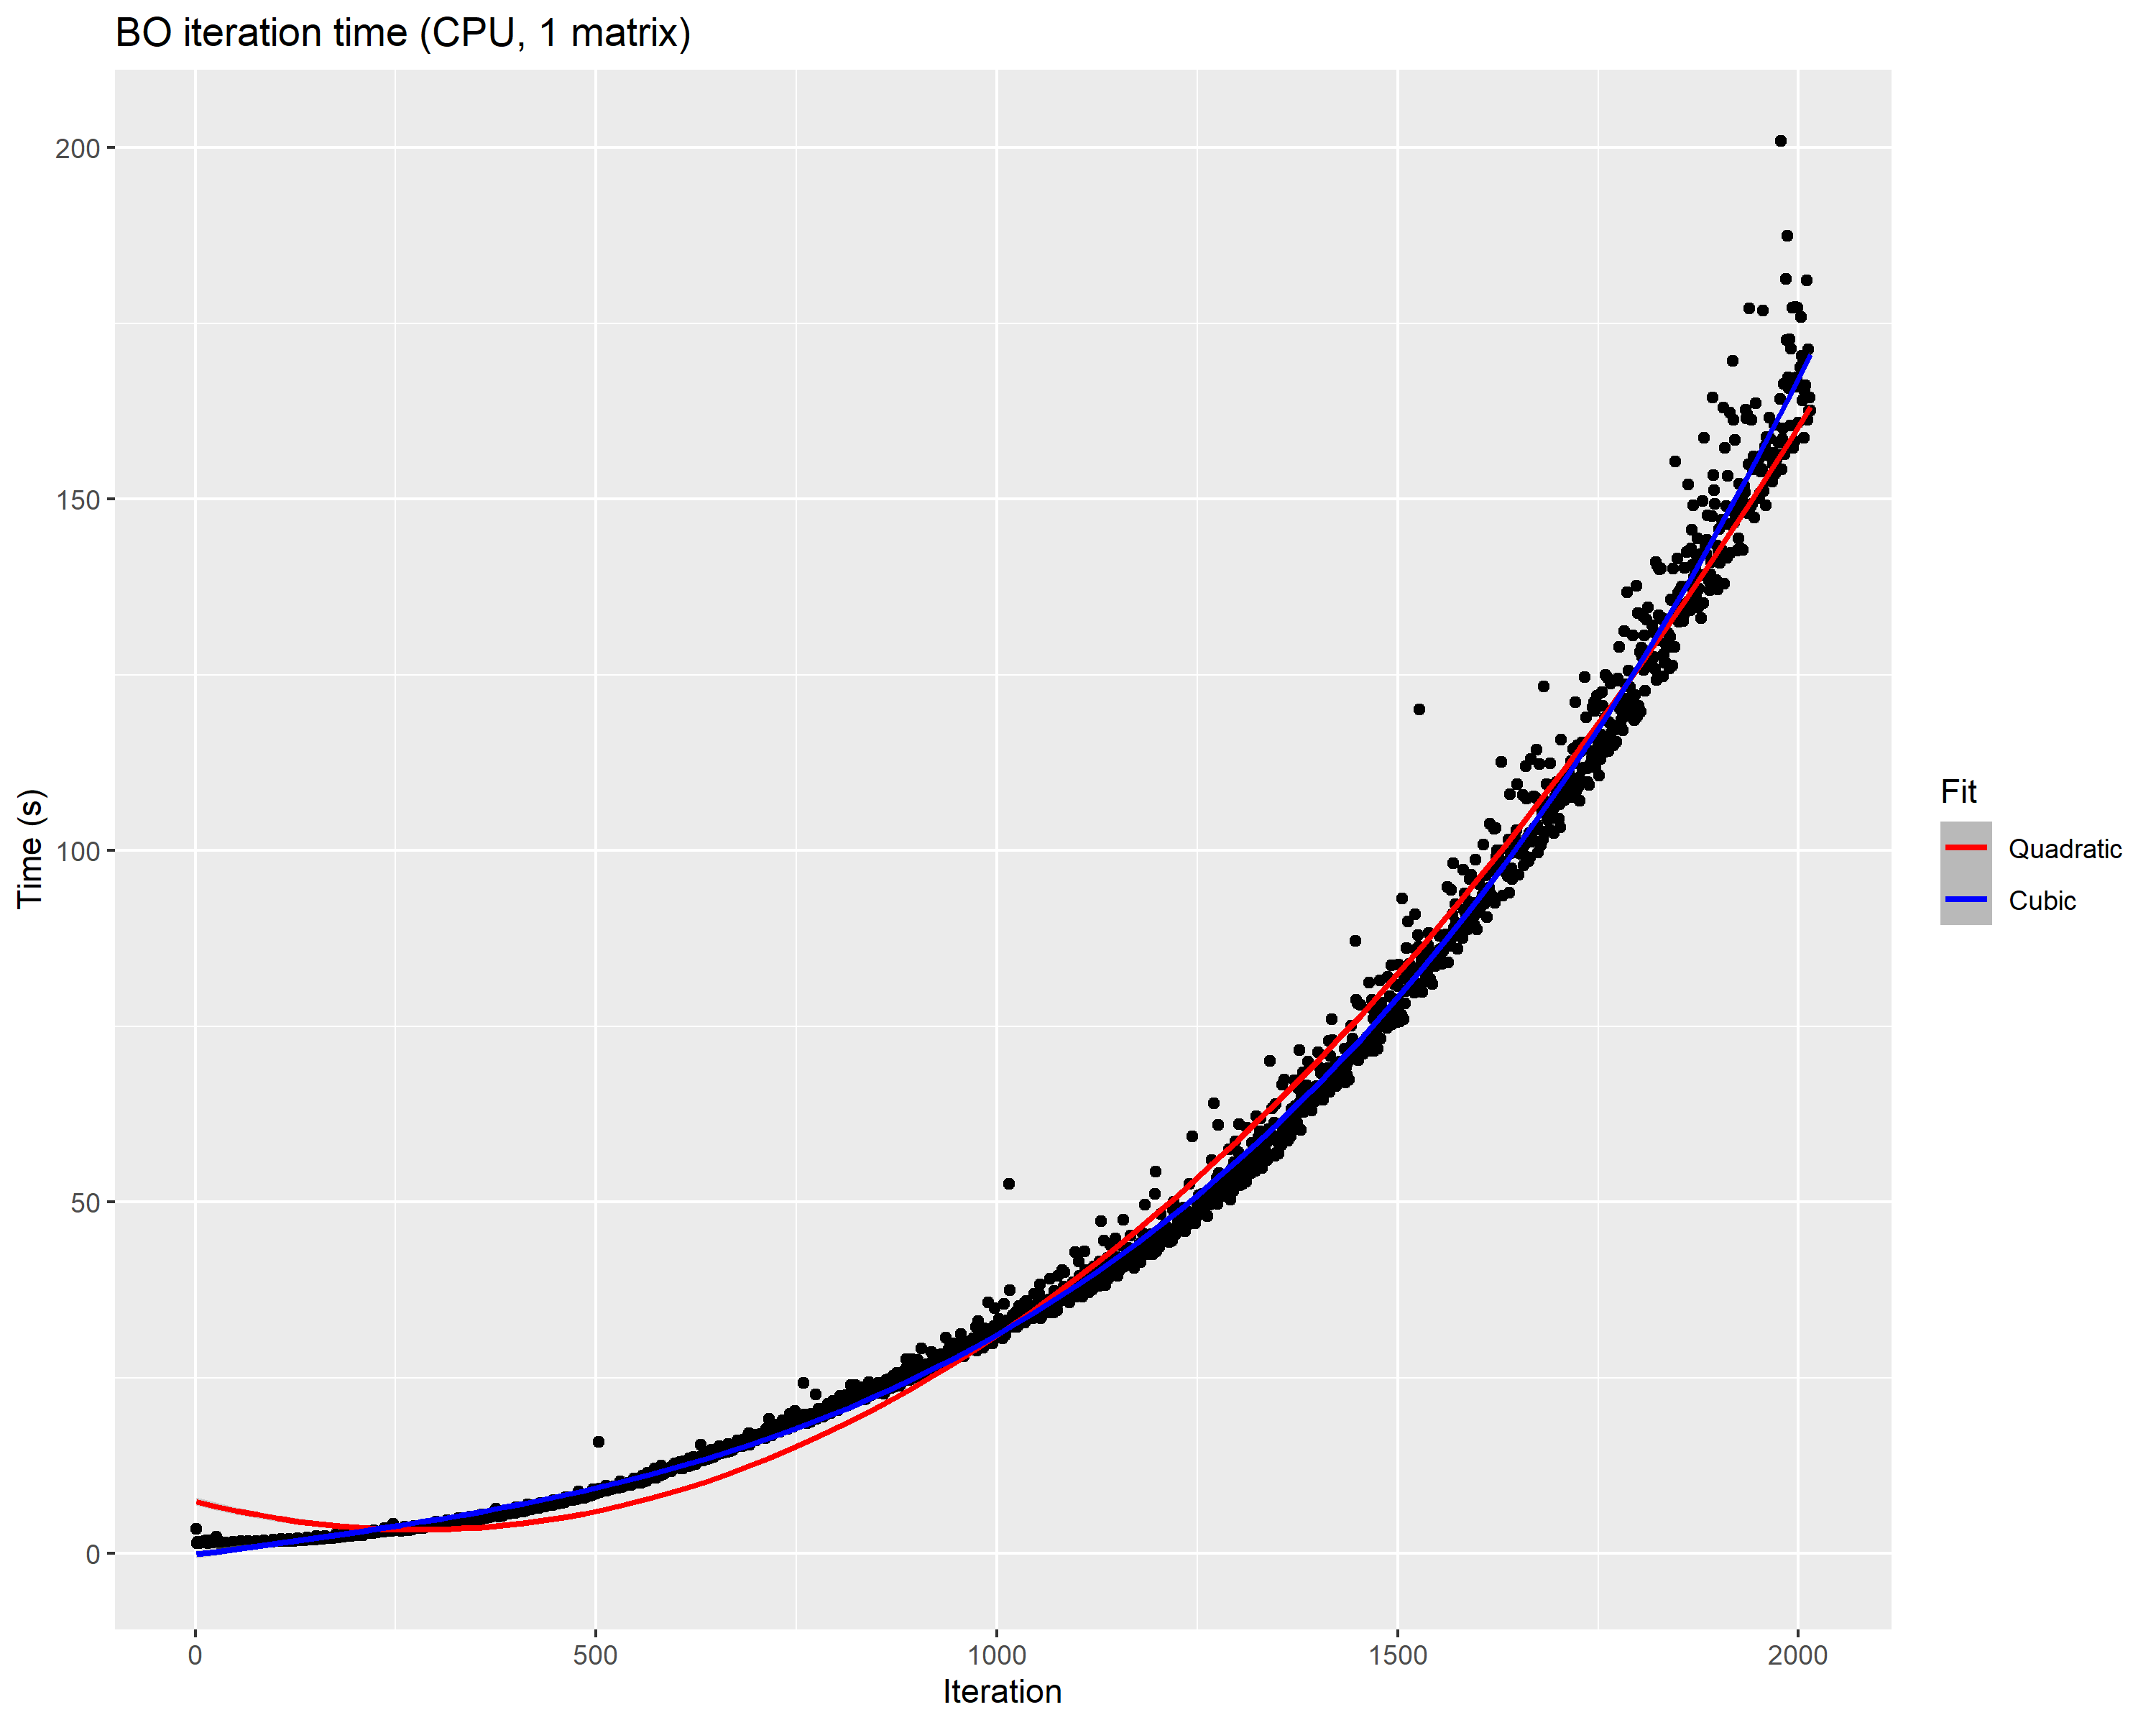
\includegraphics[width=\textwidth]{figures/bo_time_cpu_long}
\decoRule
\caption[CPU BO iteration time (2)]{CPU BO iteration time using a larger number of iterations. It is clear that the iteration times follow a cubic polynomial trend, due to the matrix inversion required in the gaussian process regression stage of the optimization procedure, as seen in figure \ref{fig:gaussian_process_regression}.}
\label{fig:bo_time_cpu_long}
\end{figure}

\begin{figure}[h!]
\centering
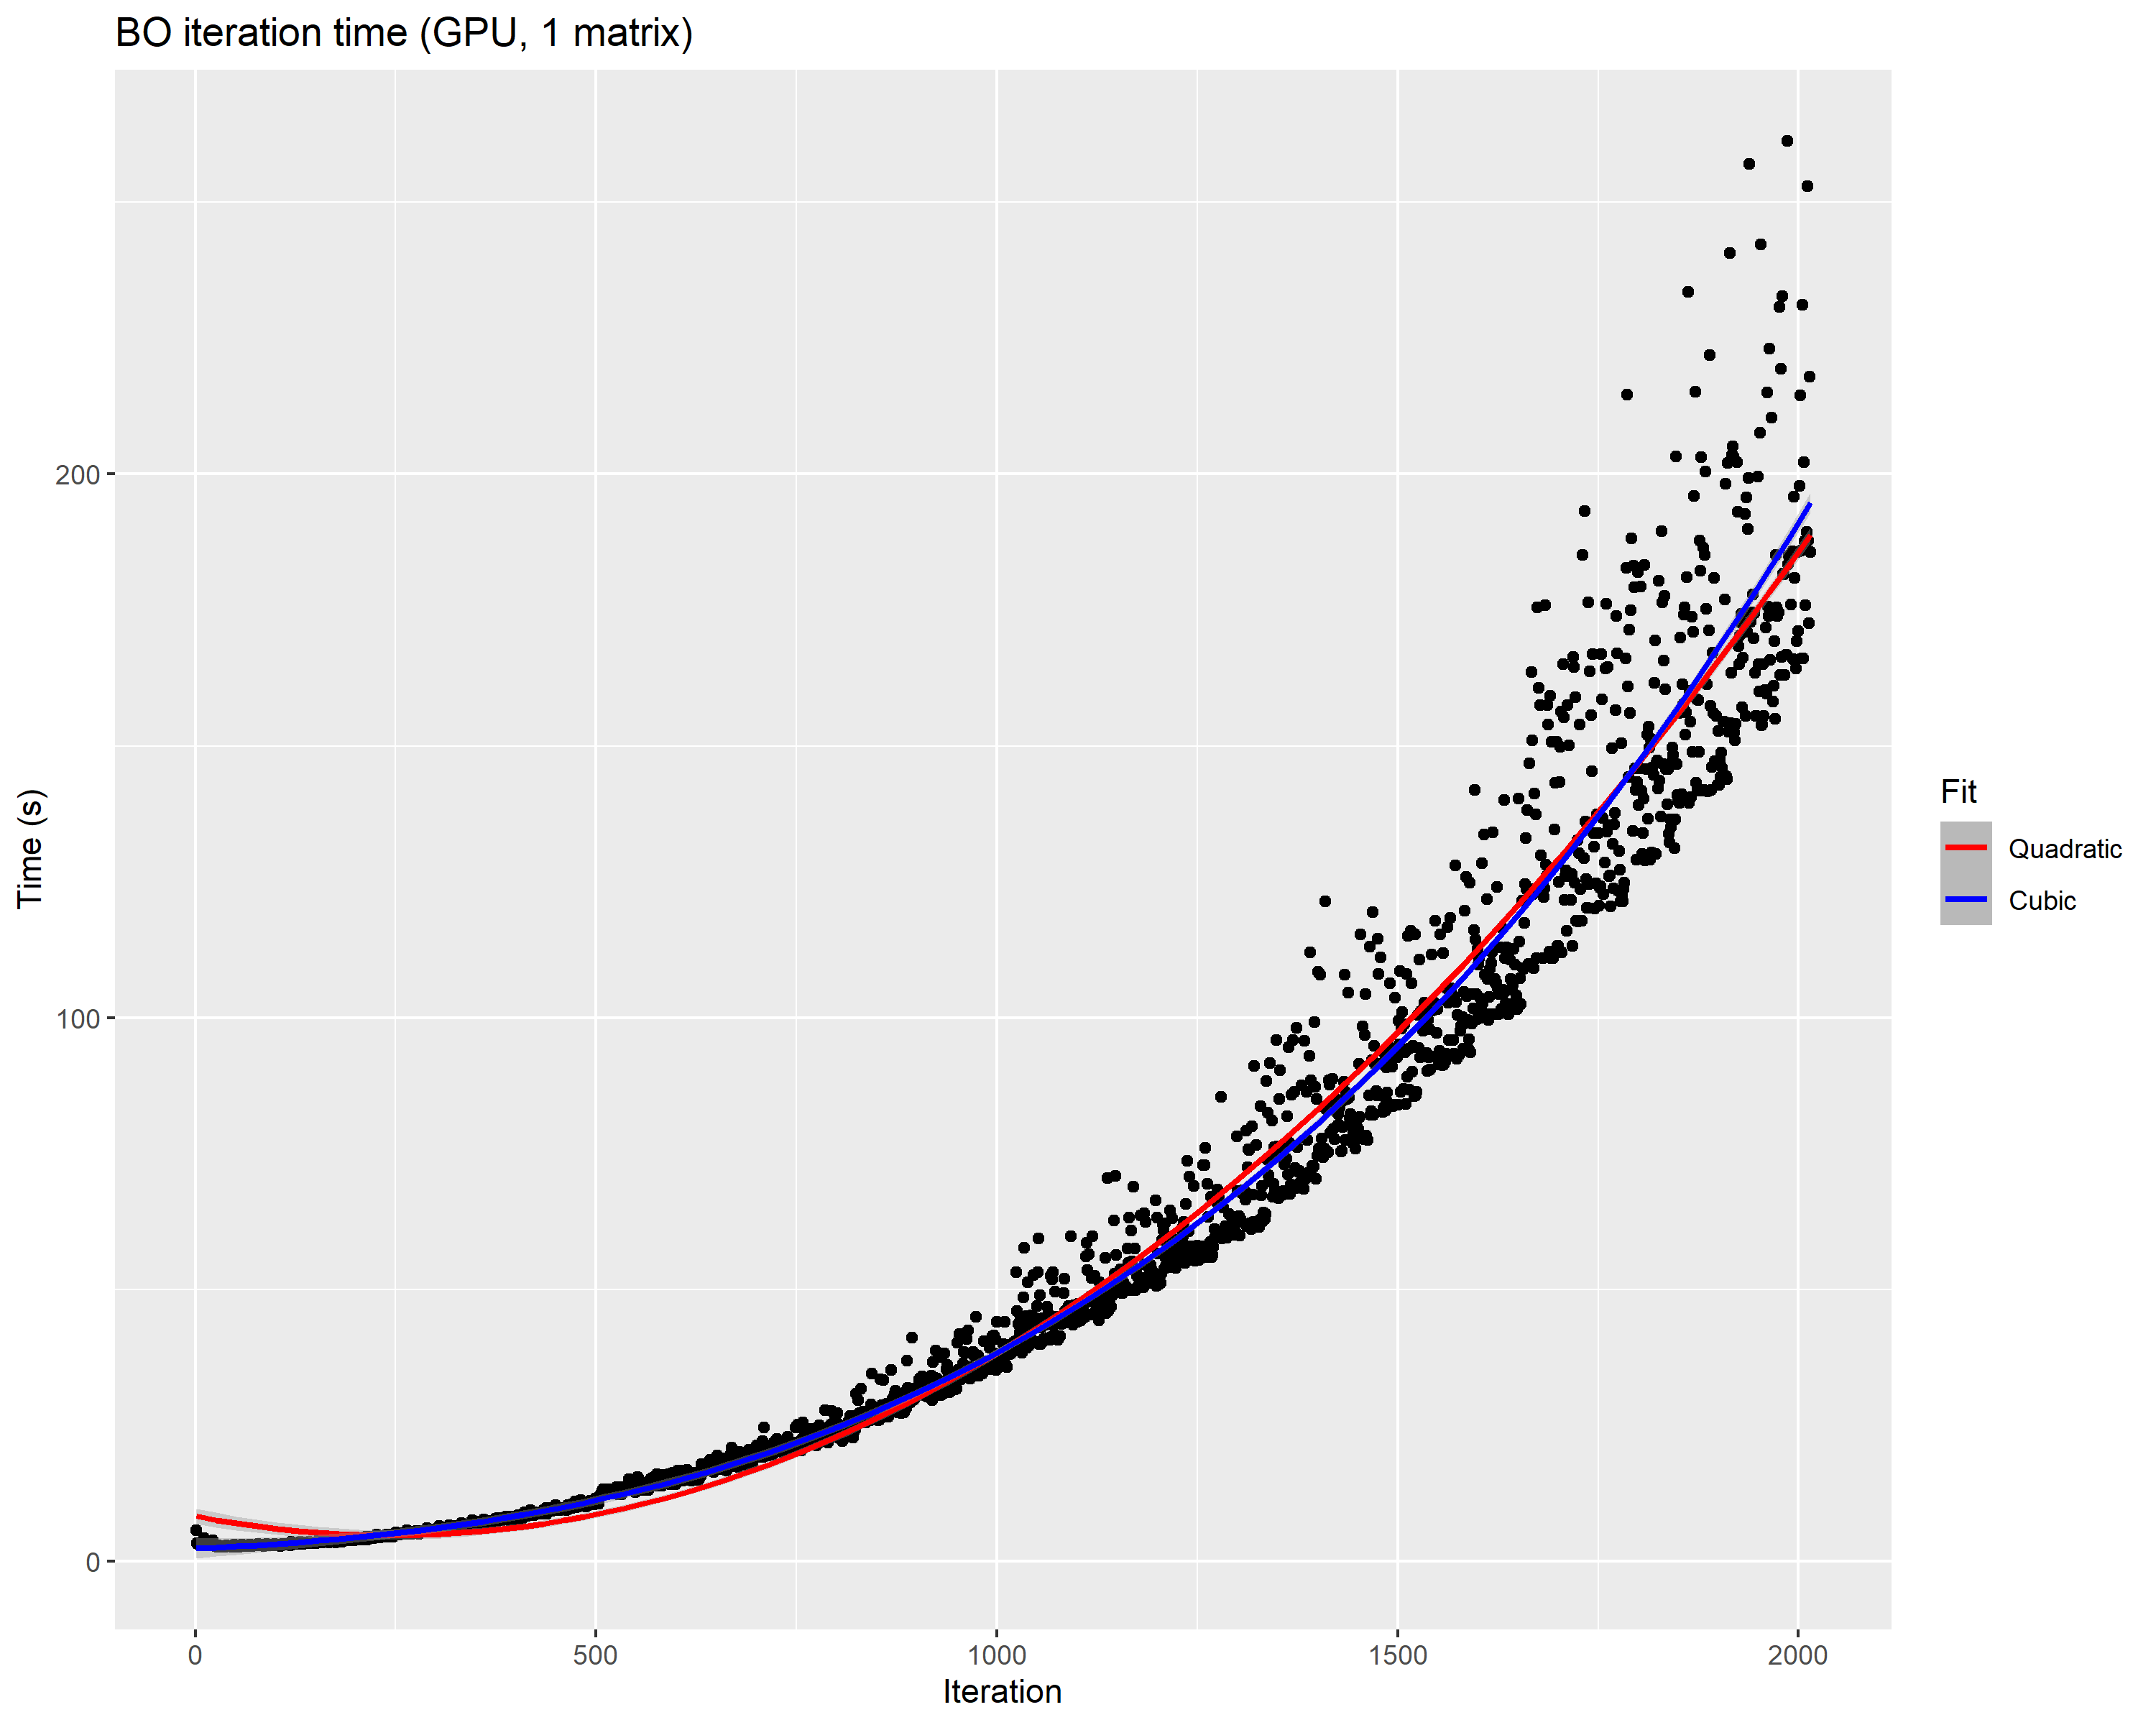
\includegraphics[width=\textwidth]{figures/bo_time_gpu_long}
\decoRule
\caption[GPU BO iteration time (2)]{GPU BO iteration time using a larger number of iterations. It is clear as well that the iteration times follow a cubic polynomial trend as the CPU optimization, but with a larger variance in the last iterations.}
\label{fig:bo_time_gpu_long}
\end{figure}

\begin{figure}[h!]
\centering
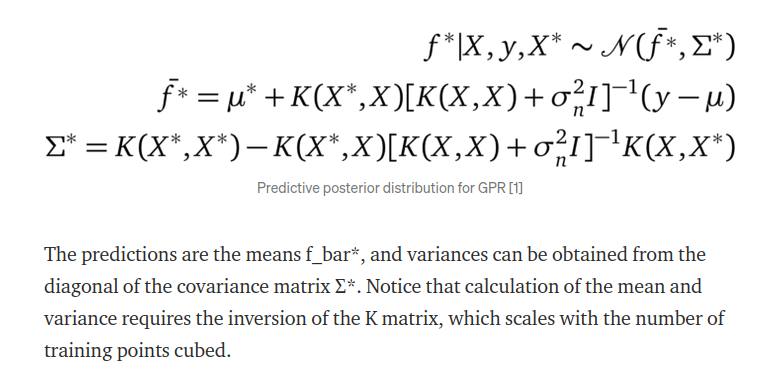
\includegraphics[width=\textwidth]{figures/gaussian_process_regression}
\decoRule
\caption[Gaussian process predictive posterior distribution]{Gaussian process predictive posterior distribution}
\label{fig:gaussian_process_regression}
\end{figure}

\begin{figure}[h!]
\centering
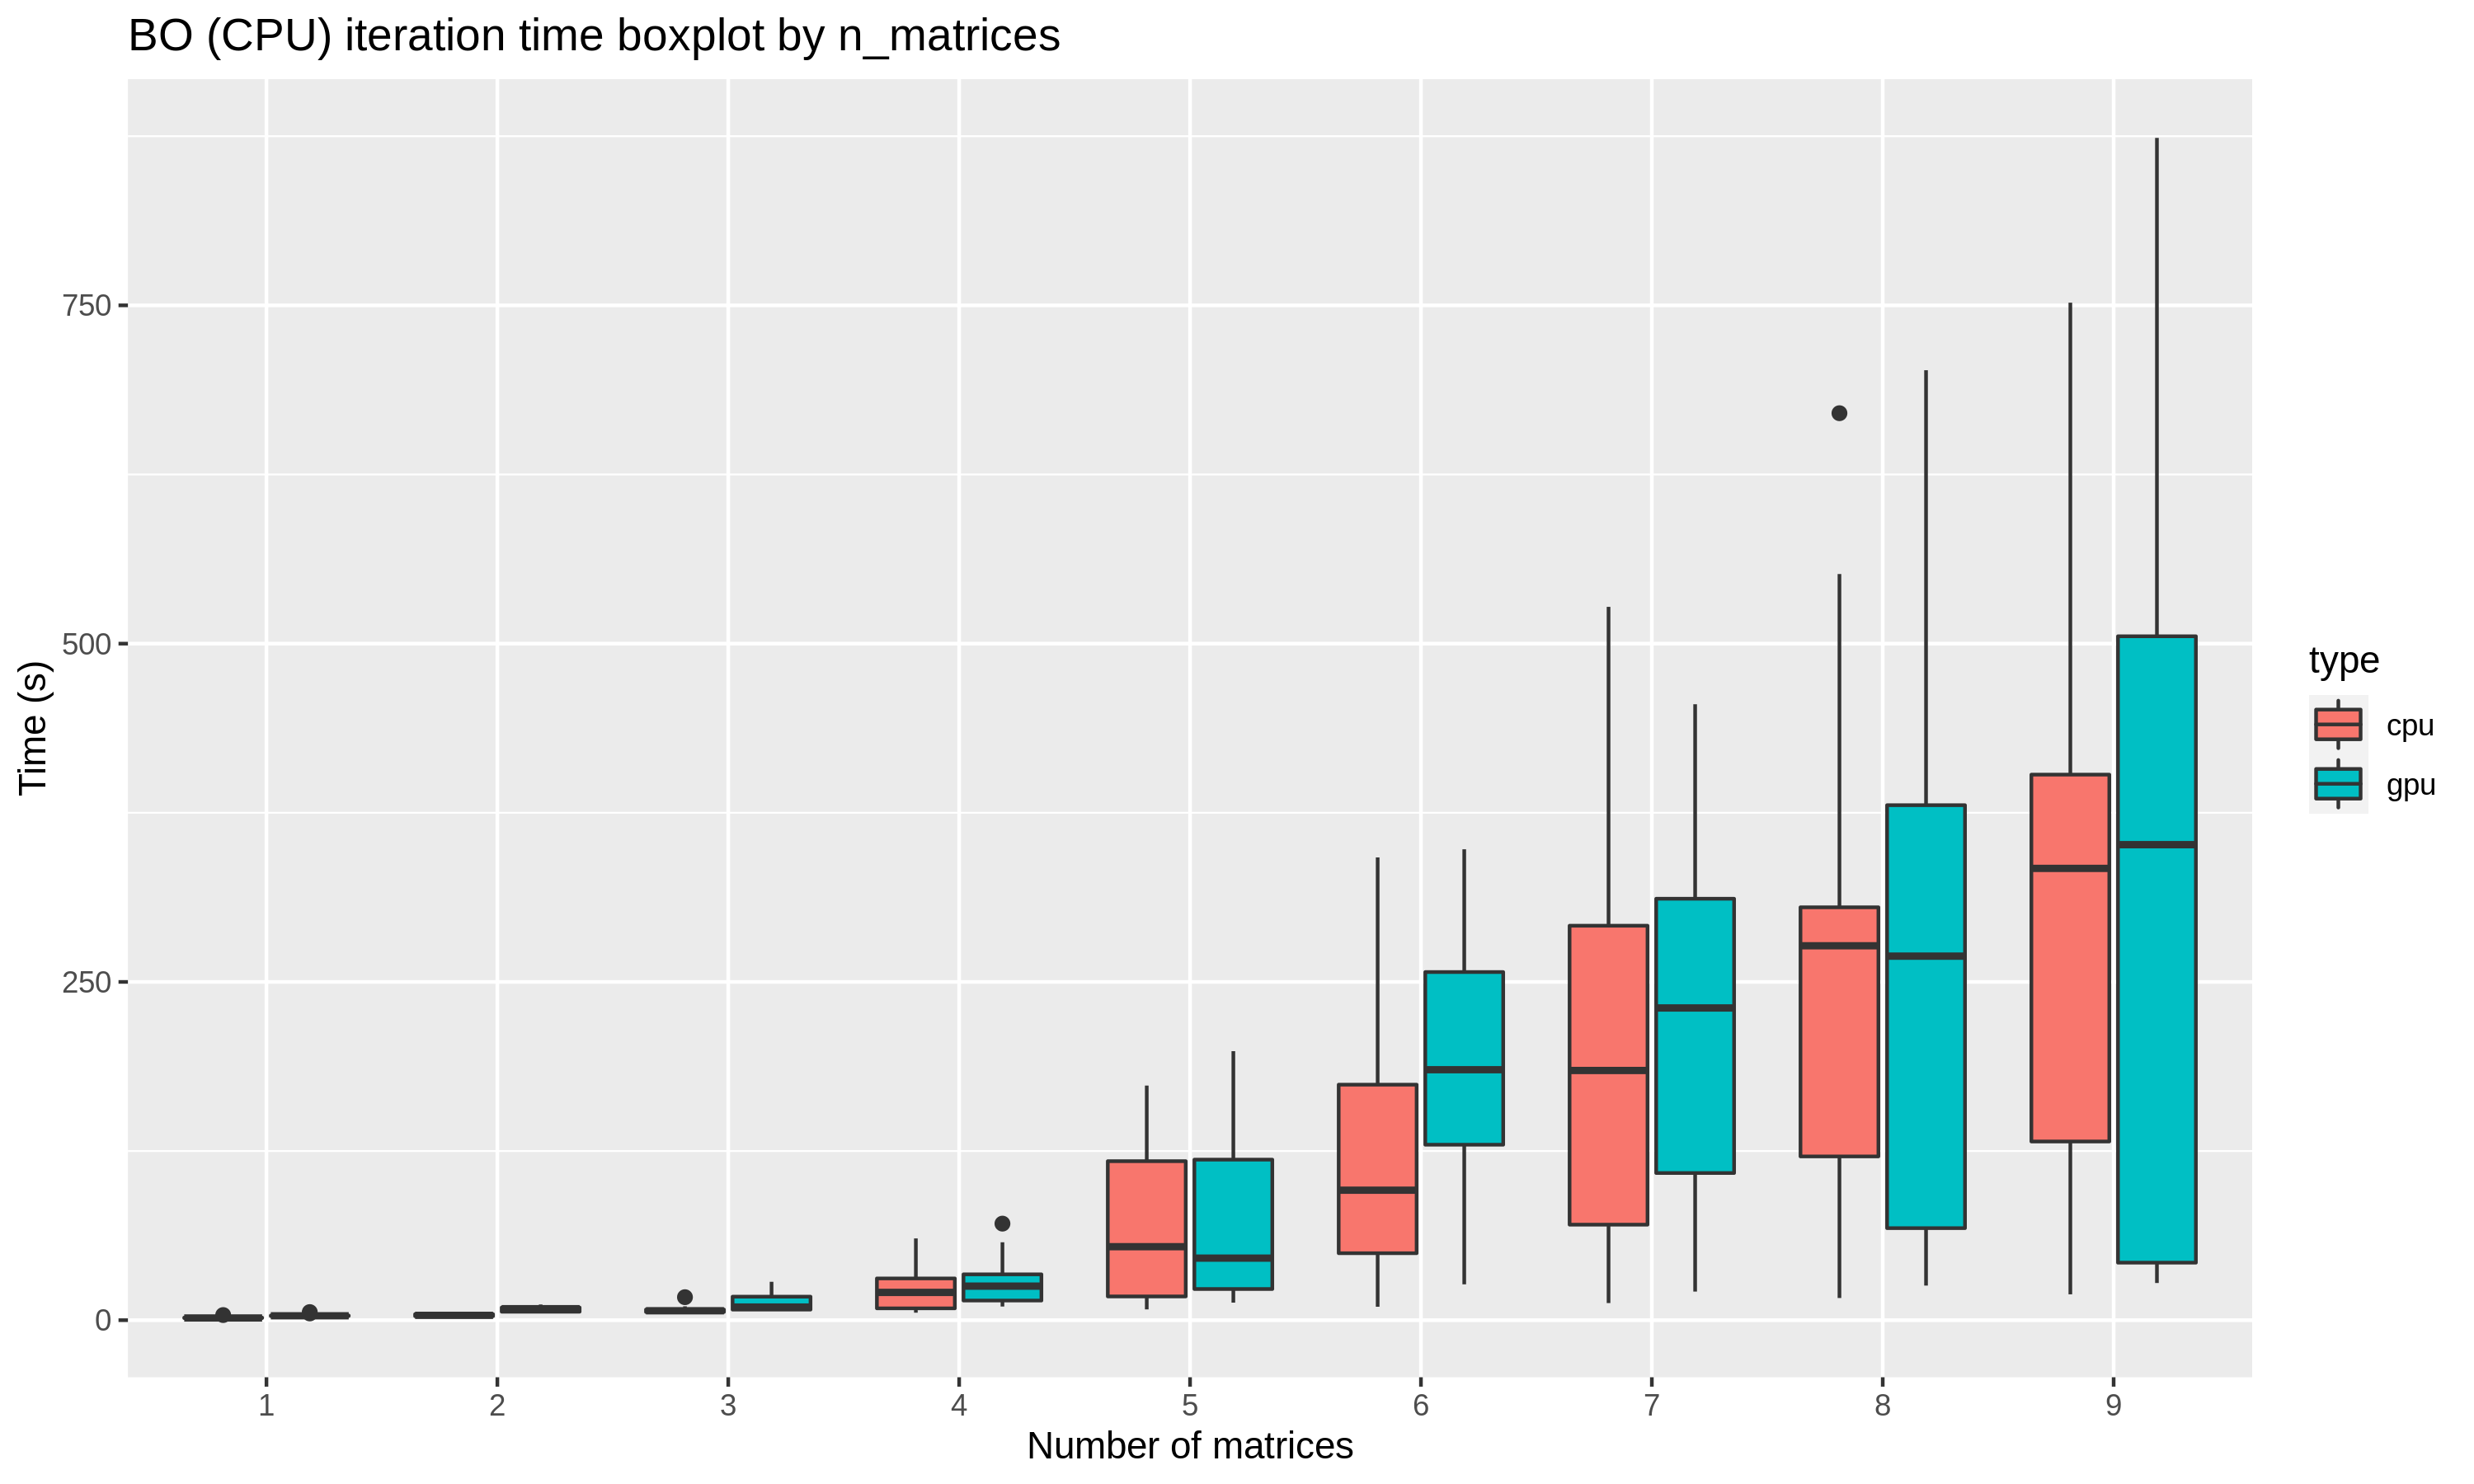
\includegraphics[width=\textwidth]{figures/bo_boxplot}
\decoRule
\caption[BO iteration time boxplot]{BO iteration time boxplot by number of matrices and computation paradigm. No significant differences between CPU/GPU are apparent; the higher values with 6 matrices using the GPU is likely to be due to chance.}
\label{fig:bo_boxplot}
\end{figure}

\begin{figure}[h!]
\centering
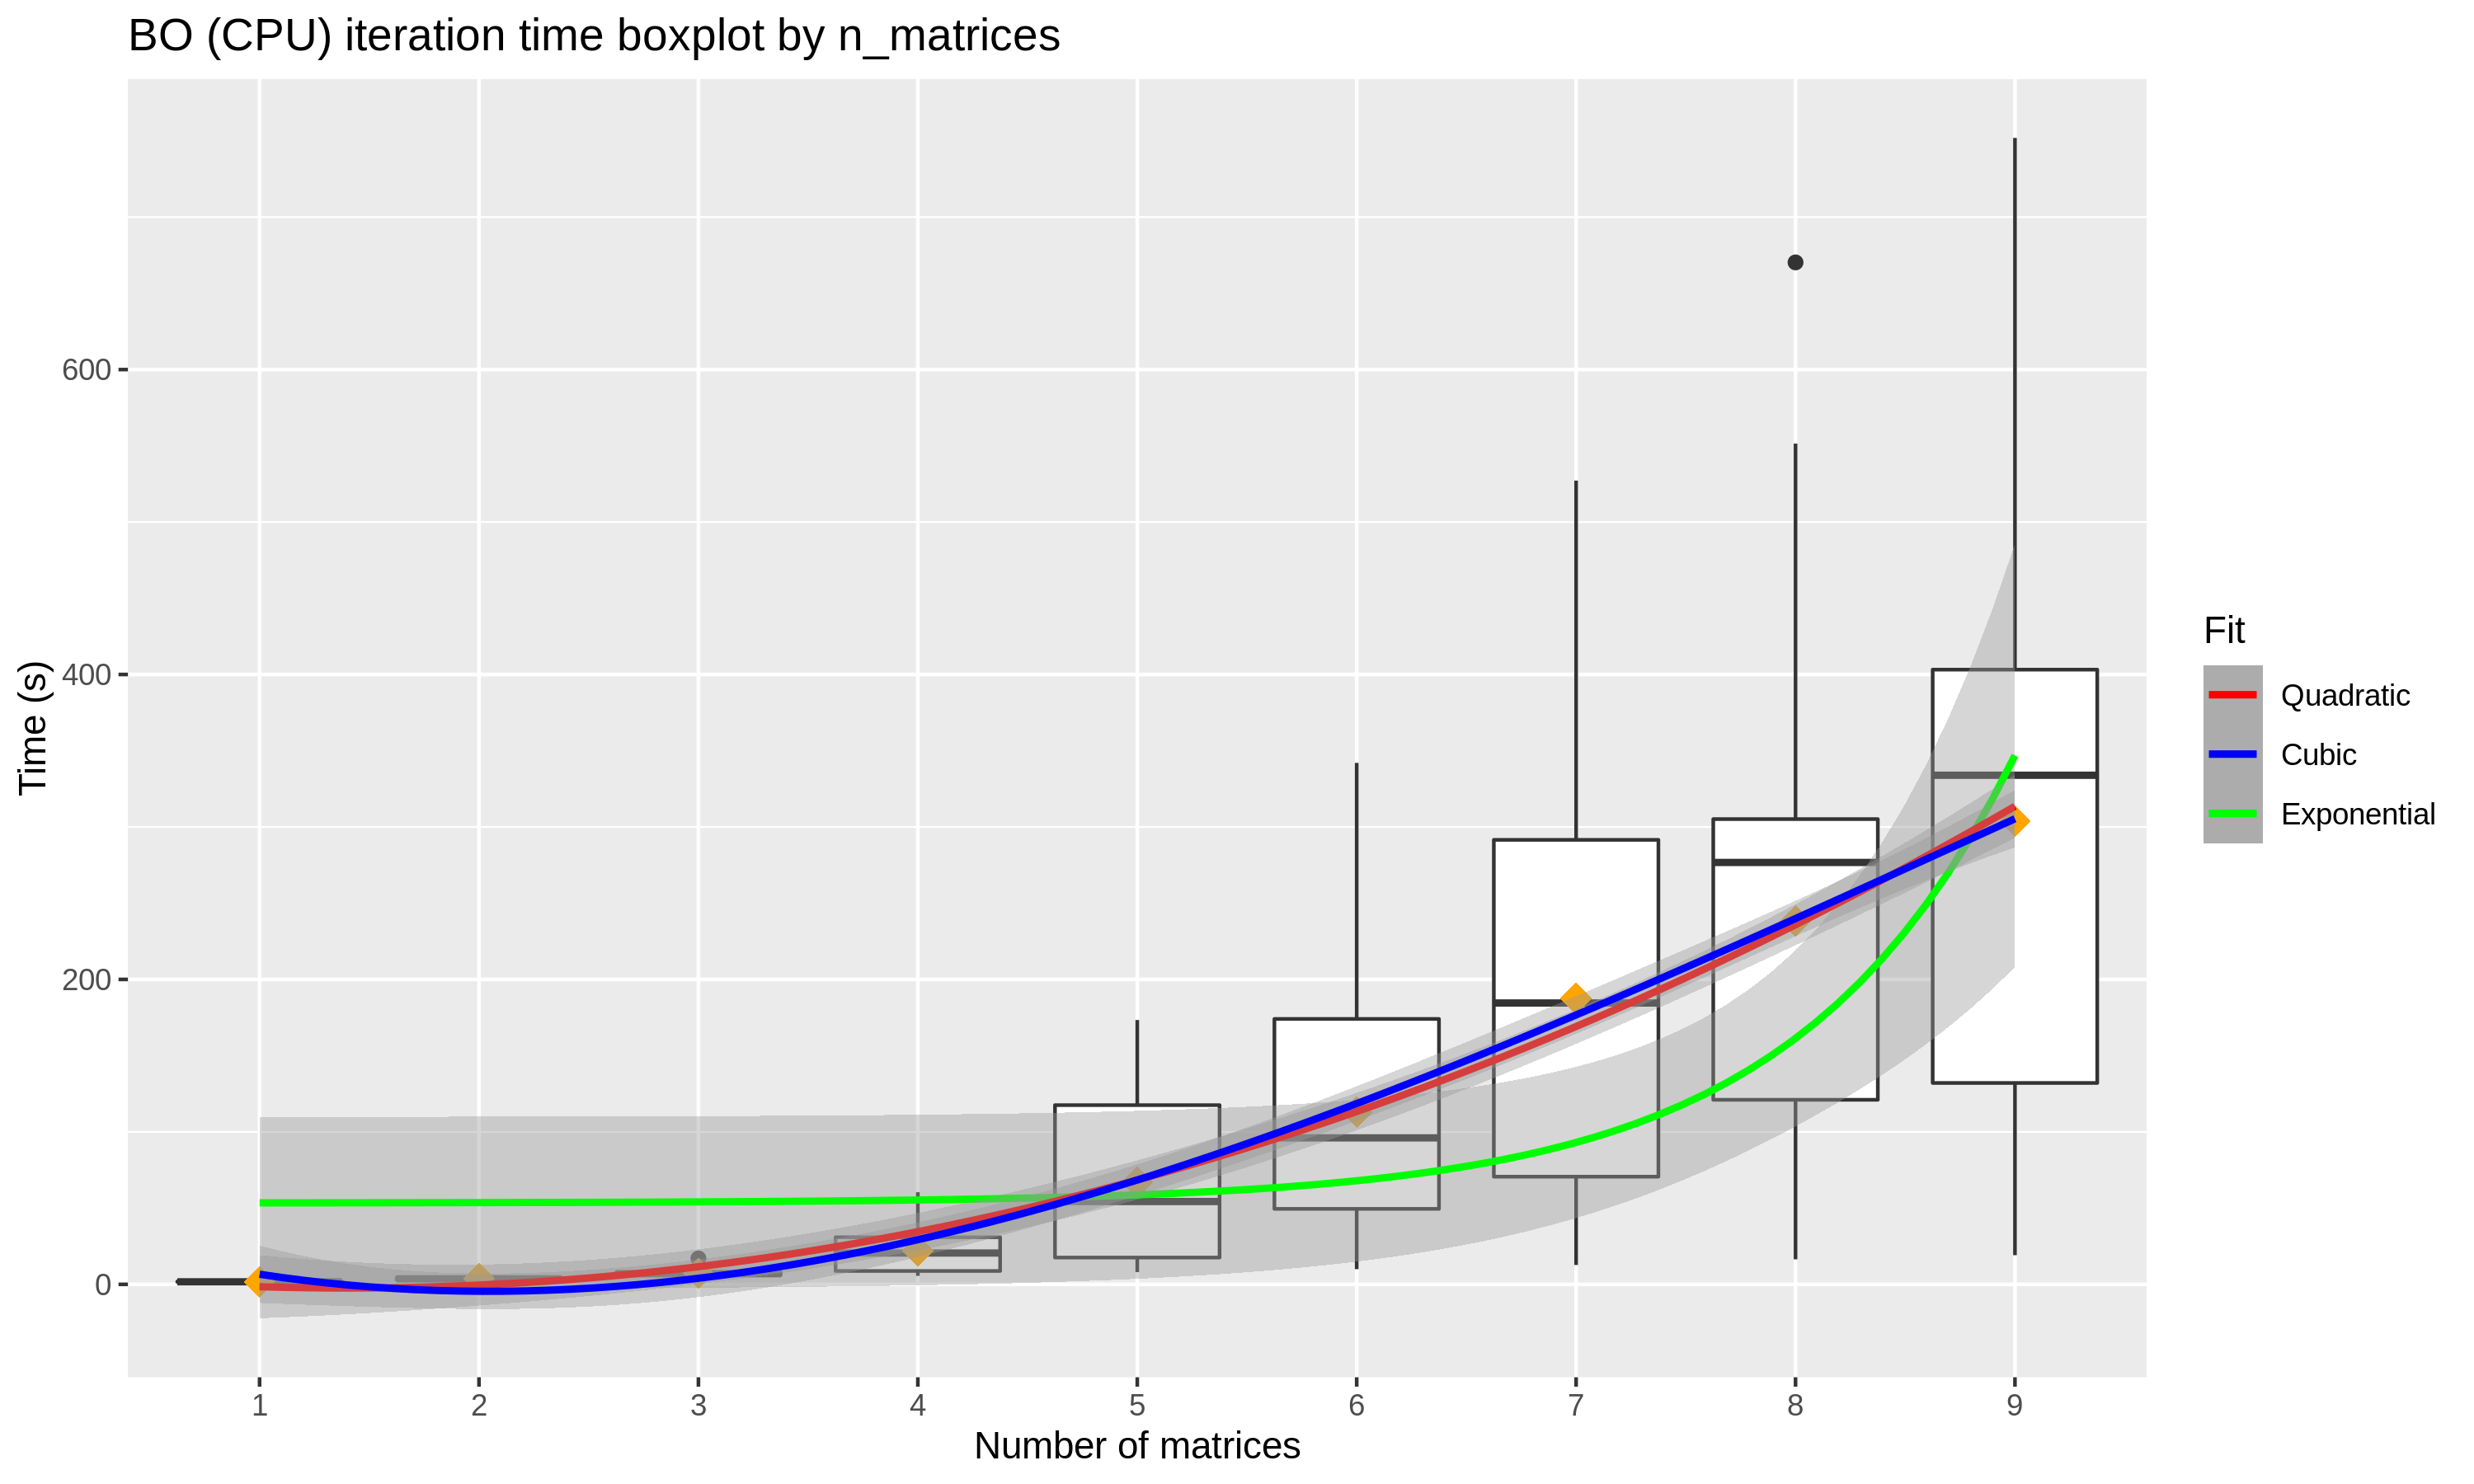
\includegraphics[width=\textwidth]{figures/bo_boxplot_cpu}
\decoRule
\caption[BO iteration time boxplot (CPU)]{CPU BO iteration time boxplot by number of matrices using the CPU with the means displayed in orange. As the number of matrices (and hence dimensions in the search space) increase the iteration time follows a quadratic trend instead of the expected exponential curve (?).}
\label{fig:bo_boxplot_cpu}
\end{figure}

\begin{figure}[h!]
\centering
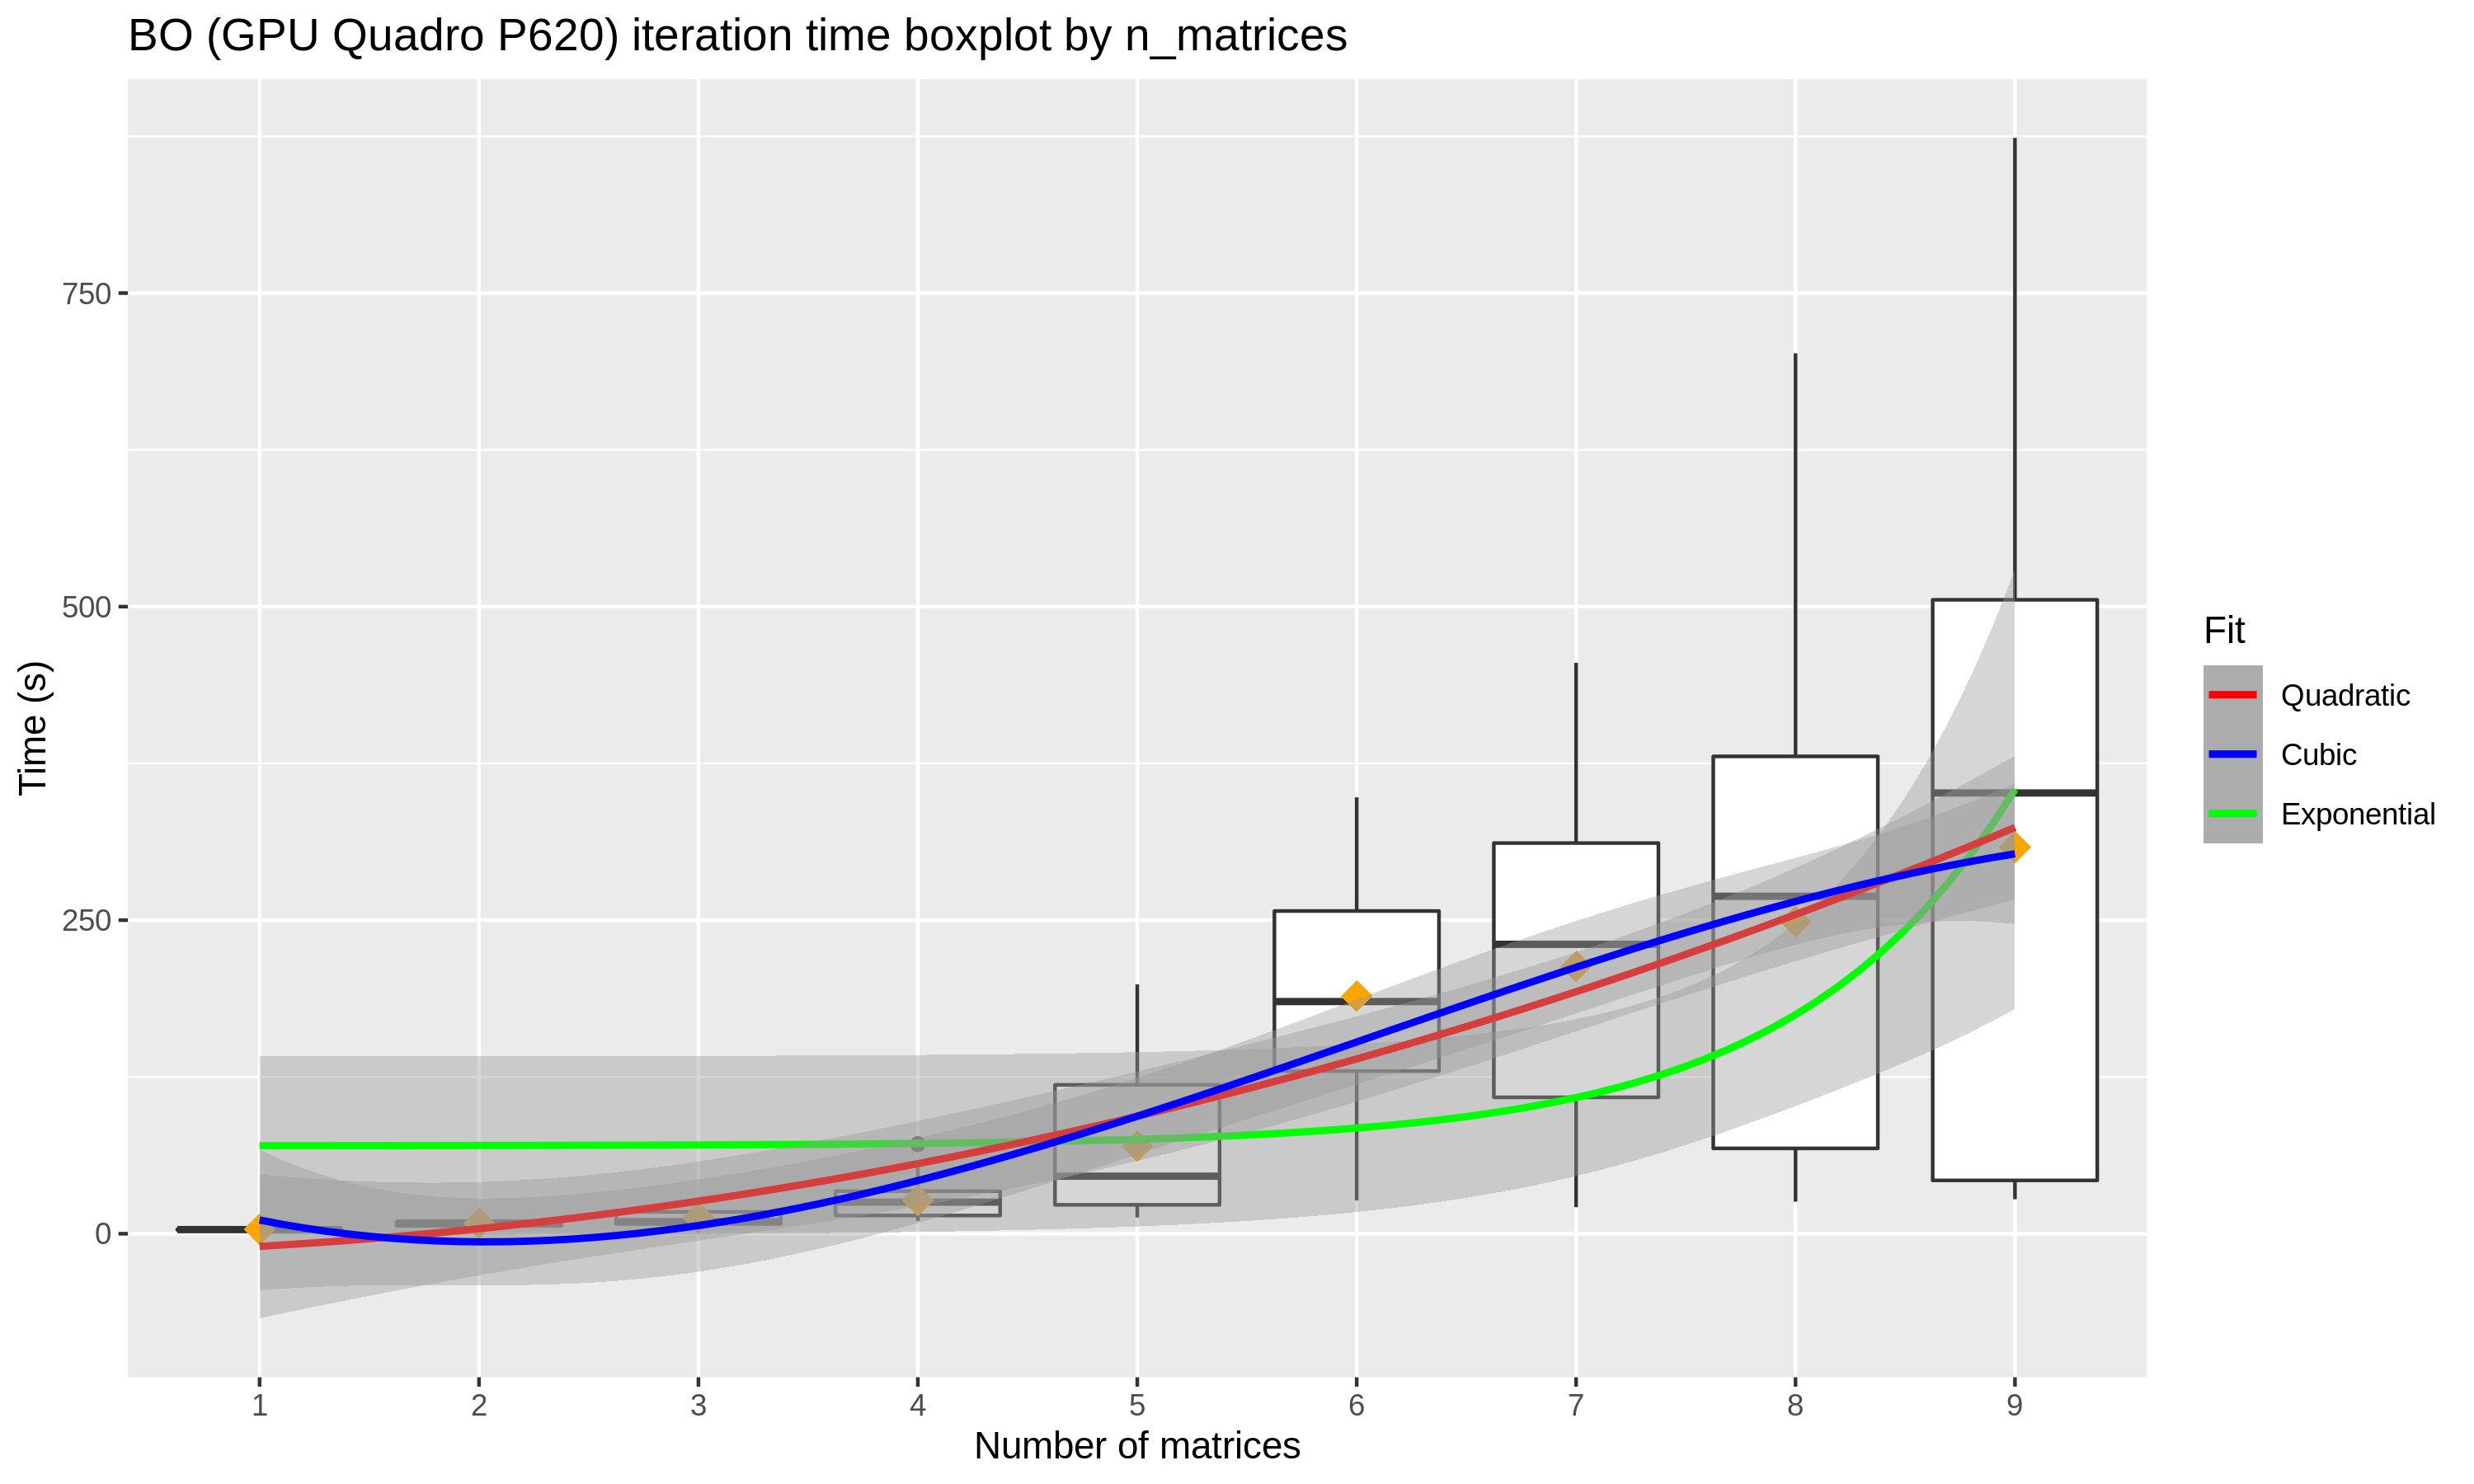
\includegraphics[width=\textwidth]{figures/bo_boxplot_gpu}
\decoRule
\caption[BO iteration time boxplot (GPU)]{GPU BO iteration time boxplot by number of matrices using the CPU with the means displayed in orange. As the number of matrices (and hence dimensions in the search space) increase the iteration time follows a quadratic trend instead of the expected exponential curve (?).}
\label{fig:bo_boxplot_gpu}
\end{figure} 
%\include{Chapters/Chapter5} 

%----------------------------------------------------------------------------------------
%	THESIS CONTENT - APPENDICES
%----------------------------------------------------------------------------------------

\appendix % Cue to tell LaTeX that the following "chapters" are Appendices

% Include the appendices of the thesis as separate files from the Appendices folder
% Uncomment the lines as you write the Appendices

%\include{Appendices/AppendixA}
%\include{Appendices/AppendixB}
%\include{Appendices/AppendixC}

%----------------------------------------------------------------------------------------
%	ABBREVIATIONS
%----------------------------------------------------------------------------------------

\begin{abbreviations}{ll} % Include a list of abbreviations (a table of two columns)
	
	\textbf{QALY} & \textbf{Q}uality \textbf{A}djusted \textbf{L}ife \textbf{Y}ear\\
	\textbf{CEA} & \textbf{C}ost \textbf{E}ffectiveness \textbf{A}nalysis\\
	\textbf{WTP} & \textbf{W}illingness \textbf{T}o \textbf{P}ay\\
	
\end{abbreviations}


%\listoffigures % Prints the list of figures

%\listoftables % Prints the list of tables

%----------------------------------------------------------------------------------------
%	BIBLIOGRAPHY
%----------------------------------------------------------------------------------------

\printbibliography[heading=bibintoc]

%----------------------------------------------------------------------------------------

\end{document}  
